\chapter{Support Material for the Combined $VH(H\rightarrow b\bar{b}/c\bar{c})$ Analysis}
\textit{This Appendix lists some additional results in support of Chapter \ref{chap-VH}.}

\section{Triggers}\label{appsec-trigger}
This section gives further details on the triggers used in the combined analysis presented in Chapter \ref{chap-VH}.
\begin{table}[!htpb]
    \begin{center}
      \scriptsize
      \resizebox{\textwidth}{!}{
        \begin{tabular}{c|c|c|c|p{7.2cm}} \hline \hline
           \textbf{ Type } & \textbf{ Trigger Name }        &     \textbf{Period}     &  \textbf{Threshold}     &     \textbf{Description}               
          \\ \hline \hline
          \multirow{5}{*}{$\etm$}  
          & HLT\_xe70\_L1XE50         &      2015               &      70 GeV                    &    
          \multirow{5}{*}{\parbox{6.6cm}{Seeded using the level L1\_XE50 (L1\_XE55) LAr and Tile calorimeter triggers, 
                          calibrated at the EM scale, with a threshold of 50(55) GeV.}} \\
          & HLT\_xe90\_mht\_L1XE50         &      2016 (A-D3)               &      90 GeV                    &     \\
          & HLT\_xe110\_mht\_L1XE50        &      2016 ($\geq$ D4)              &      110 GeV                   &     \\
          & HLT\_xe110\_pufit\_L1XE55        &      2017               &      110 GeV                   &    \\
          & HLT\_xe110\_pufit\_xe70\_L1XE50        &      2018               &      110 GeV                   &    \\
          \hline \hline
          \multirow{7}{*}{Electron}  
          & HLT\_e24\_lhmedium\_L1EM20VH  &  2015  &   24 GeV    &    Seeded using L1 EM20VH level 1 trigger calibrated at the EM scale with a threshold of 20 GeV, require likelihood medium ID.\\
          & HLT\_e60\_lhmedium            &  2015  &   60 GeV    &    Require likelihood medium ID.\\
          & HLT\_e120\_lhloose            &  2015  &  120 GeV    &    Require likelihood loose ID.\\
          & HLT\_e26\_lhtight\_nod0\_ivarloose  &      2016 -- 2018         &         26 GeV     &    Tight likelihood ID required, alignment-robust likelihood tune with no d0 information used, and variable loose isolation required\\
          & HLT\_e60\_lhmedium(\_nod0)           &      2016 -- 2018        &         60 GeV     &    Medium ID likelihood required\\
          & HLT\_e140\_lhloose(\_nod0)           &      2016 -- 2018        &         140 GeV    &    Loose ID likelihood required\\
          & HLT\_e300\_etcut                     &      2018                &         300 GeV    &    No ID requirements. \\
          \hline \hline
          \multirow{3}{*}{Muon}  
          & HLT\_mu20\_iloose\_L1MU15      &      2015           &  20 GeV &   Seeded using L1MU15 level 1 trigger with a threshold of 15 GeV, and requiring loose isolation requirements.\\
          & HLT\_mu50\                     &      2015 -- 2018   &  50 GeV &   No isolation requirements. \\
          & HLT\_mu26\_ivarmedium          &      2016 -- 2018   &  26 GeV &   Variable cone medium isolation requirements \\
          \hline \hline
        \end{tabular}
      }
      \caption{Triggers used during the 2015-2018 data collection period, from the internal documentation.
               For the HLT that L1 trigger is not mentioned, the default L1 trigger is used. 
               The default L1 trigger is EM22VHI or EM24VHI for single electron, 
               MU20 or MU21 for single muon, depends on the data taken period
               \cite{TwikiTriggerNamingRun2}. }
      \label{tab:trigs2015_to_2018}
    \end{center}
  \end{table}

\section{Flavour Tagging Calibrations}\label{appsec-vh-ftagcal}
\begin{figure}
    \centering
         \subfigure{\label{subfig:FTAG_calibration_resolved_B}}{%
           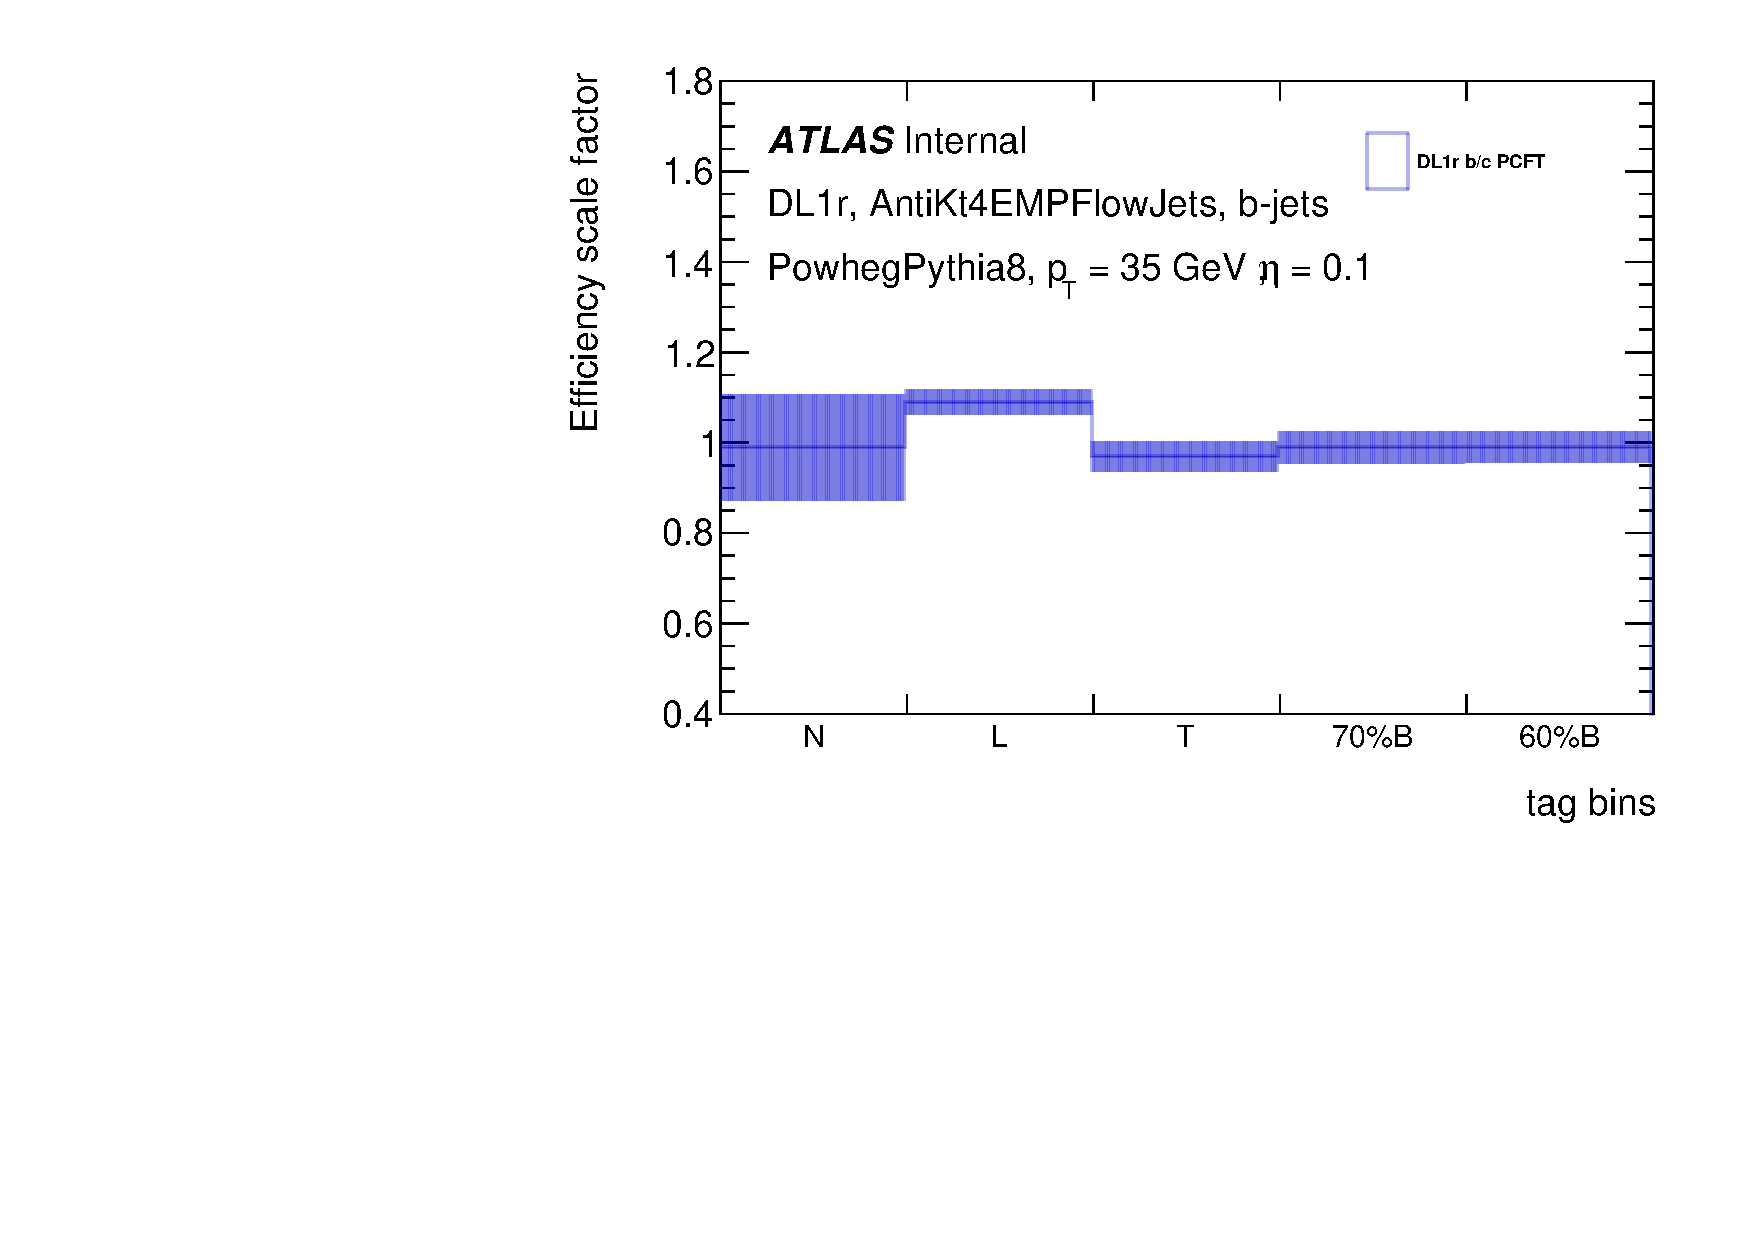
\includegraphics[width=0.4\linewidth]{Images/VH/Obj/FTAGCalib/ftagres/DL1r_AntiKt4EMPFlowJets_BTagging201903_Continuous2D_B_410470_30_eta01.pdf}}
         \subfigure{\label{subfig:FTAG_calibration_resolved_C}}{%
           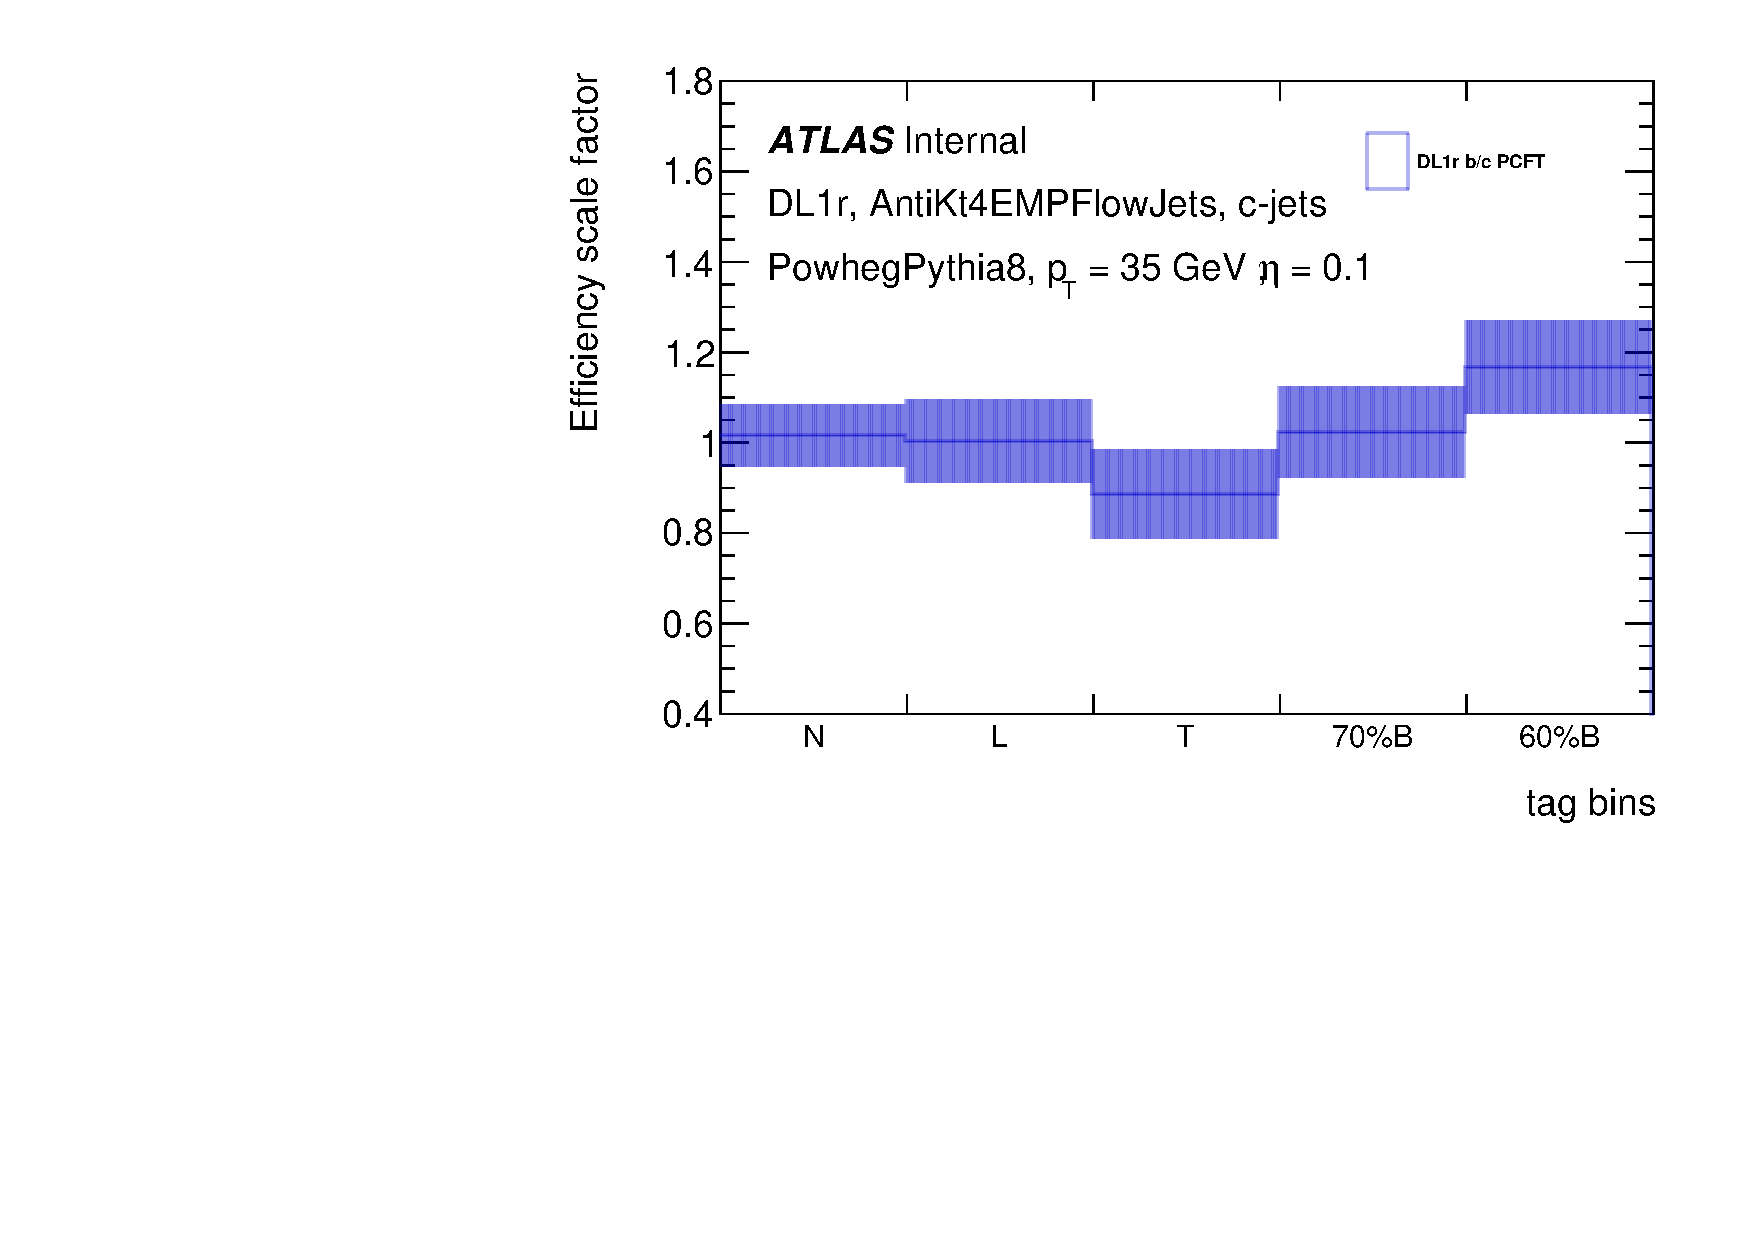
\includegraphics[width=0.4\linewidth]{Images/VH/Obj/FTAGCalib/ftagres/DL1r_AntiKt4EMPFlowJets_BTagging201903_Continuous2D_C_410470_30_eta01.pdf}}\\
         \subfigure{\label{subfig:FTAG_calibration_resolved_Light}}{%
           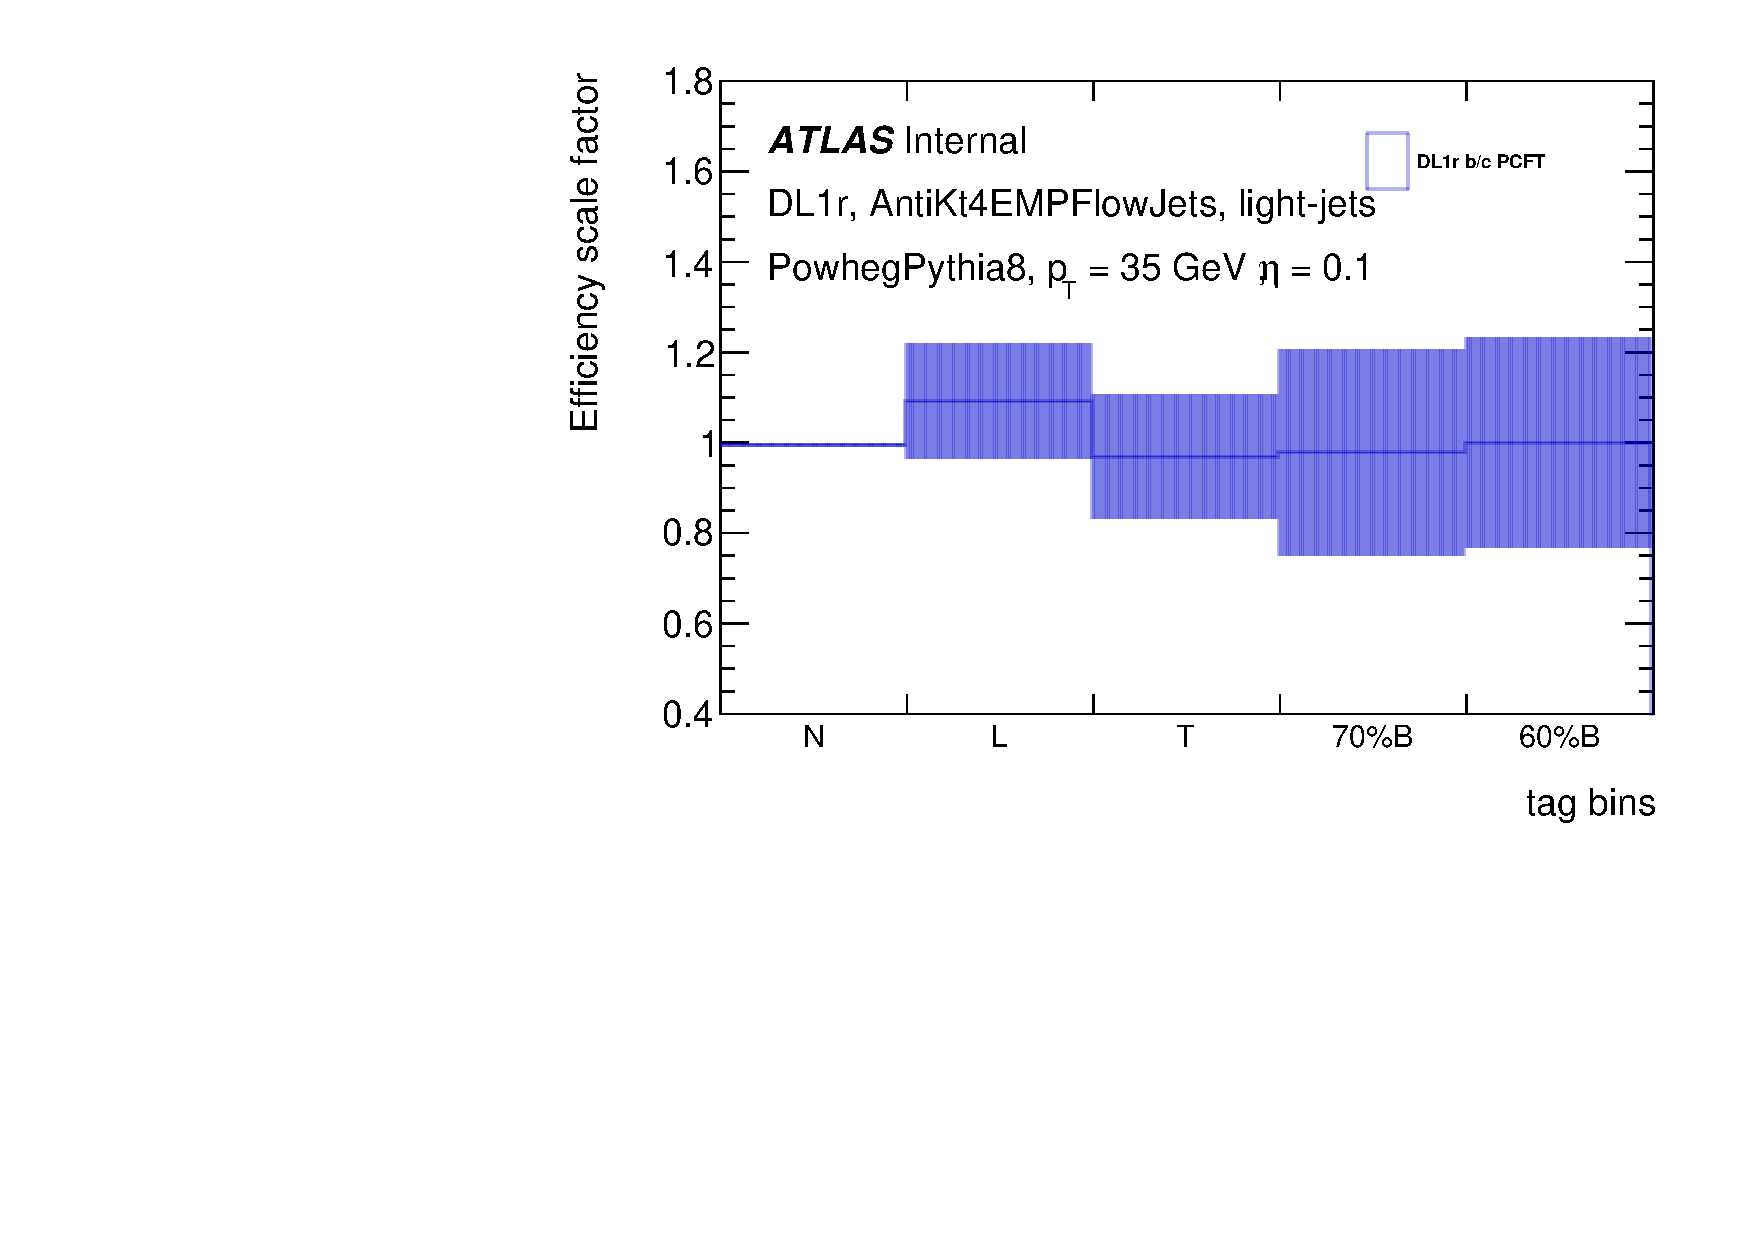
\includegraphics[width=0.4\linewidth]{Images/VH/Obj/FTAGCalib/ftagres/DL1r_AntiKt4EMPFlowJets_BTagging201903_Continuous2D_Light_410470_30_eta01.pdf}}
         \subfigure{\label{subfig:FTAG_calibration_resolved_T}}{%
           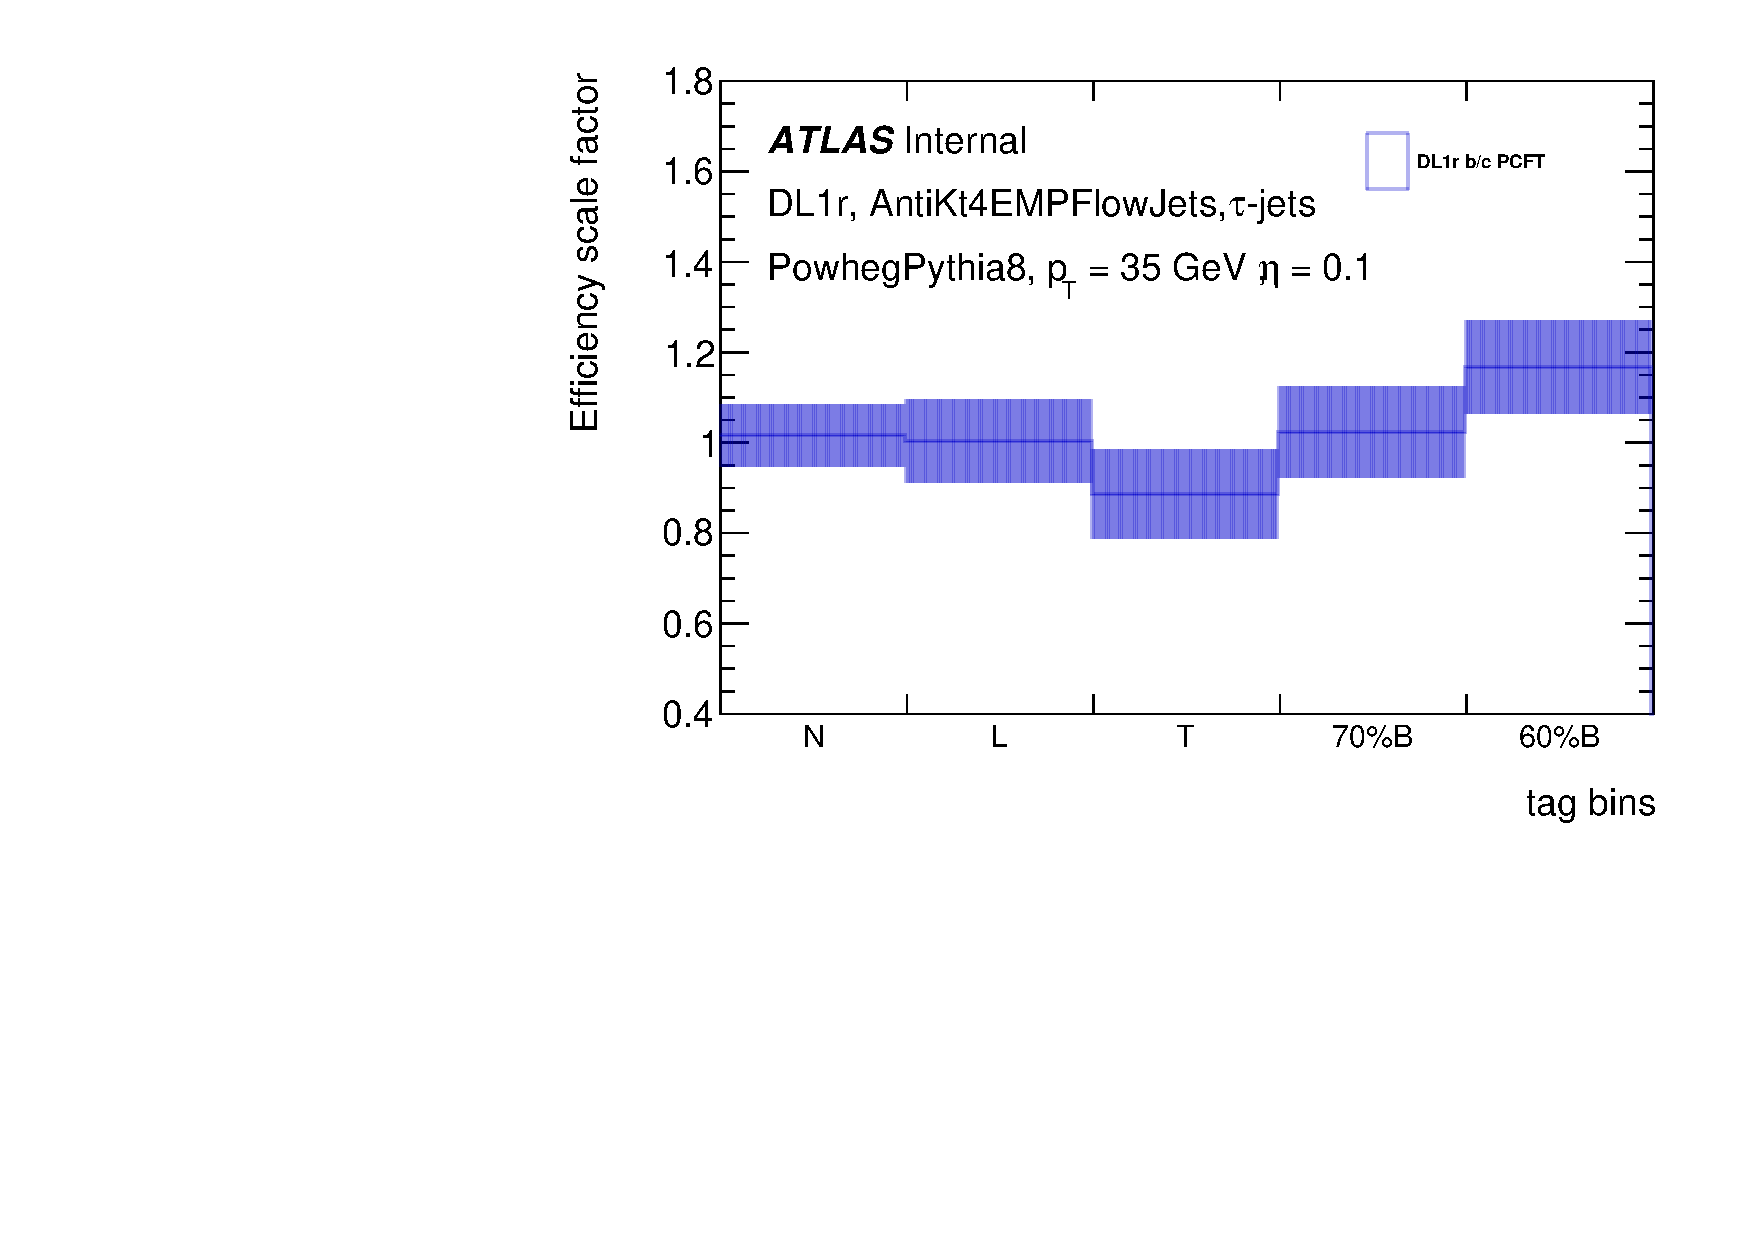
\includegraphics[width=0.4\linewidth]{Images/VH/Obj/FTAGCalib/ftagres/DL1r_AntiKt4EMPFlowJets_BTagging201903_Continuous2D_T_410470_30_eta01.pdf}}
       \caption{%
       Efficiency scale factor calibration results of the DL1r \gls{pcft} tagger on PowhegPythia8 \ttb samples for the resolved regime of the \vhbc. The scale factors of $\tau$-jets are from $c$-jet calibration. From the internal documentation.
       }%
       \label{appfig:FTAG_calibration_resolved}
   \end{figure}
   
   \begin{figure}
     \centering
         \subfigure{\label{subfig:FTAG_calibration_boosted_B}}{%
           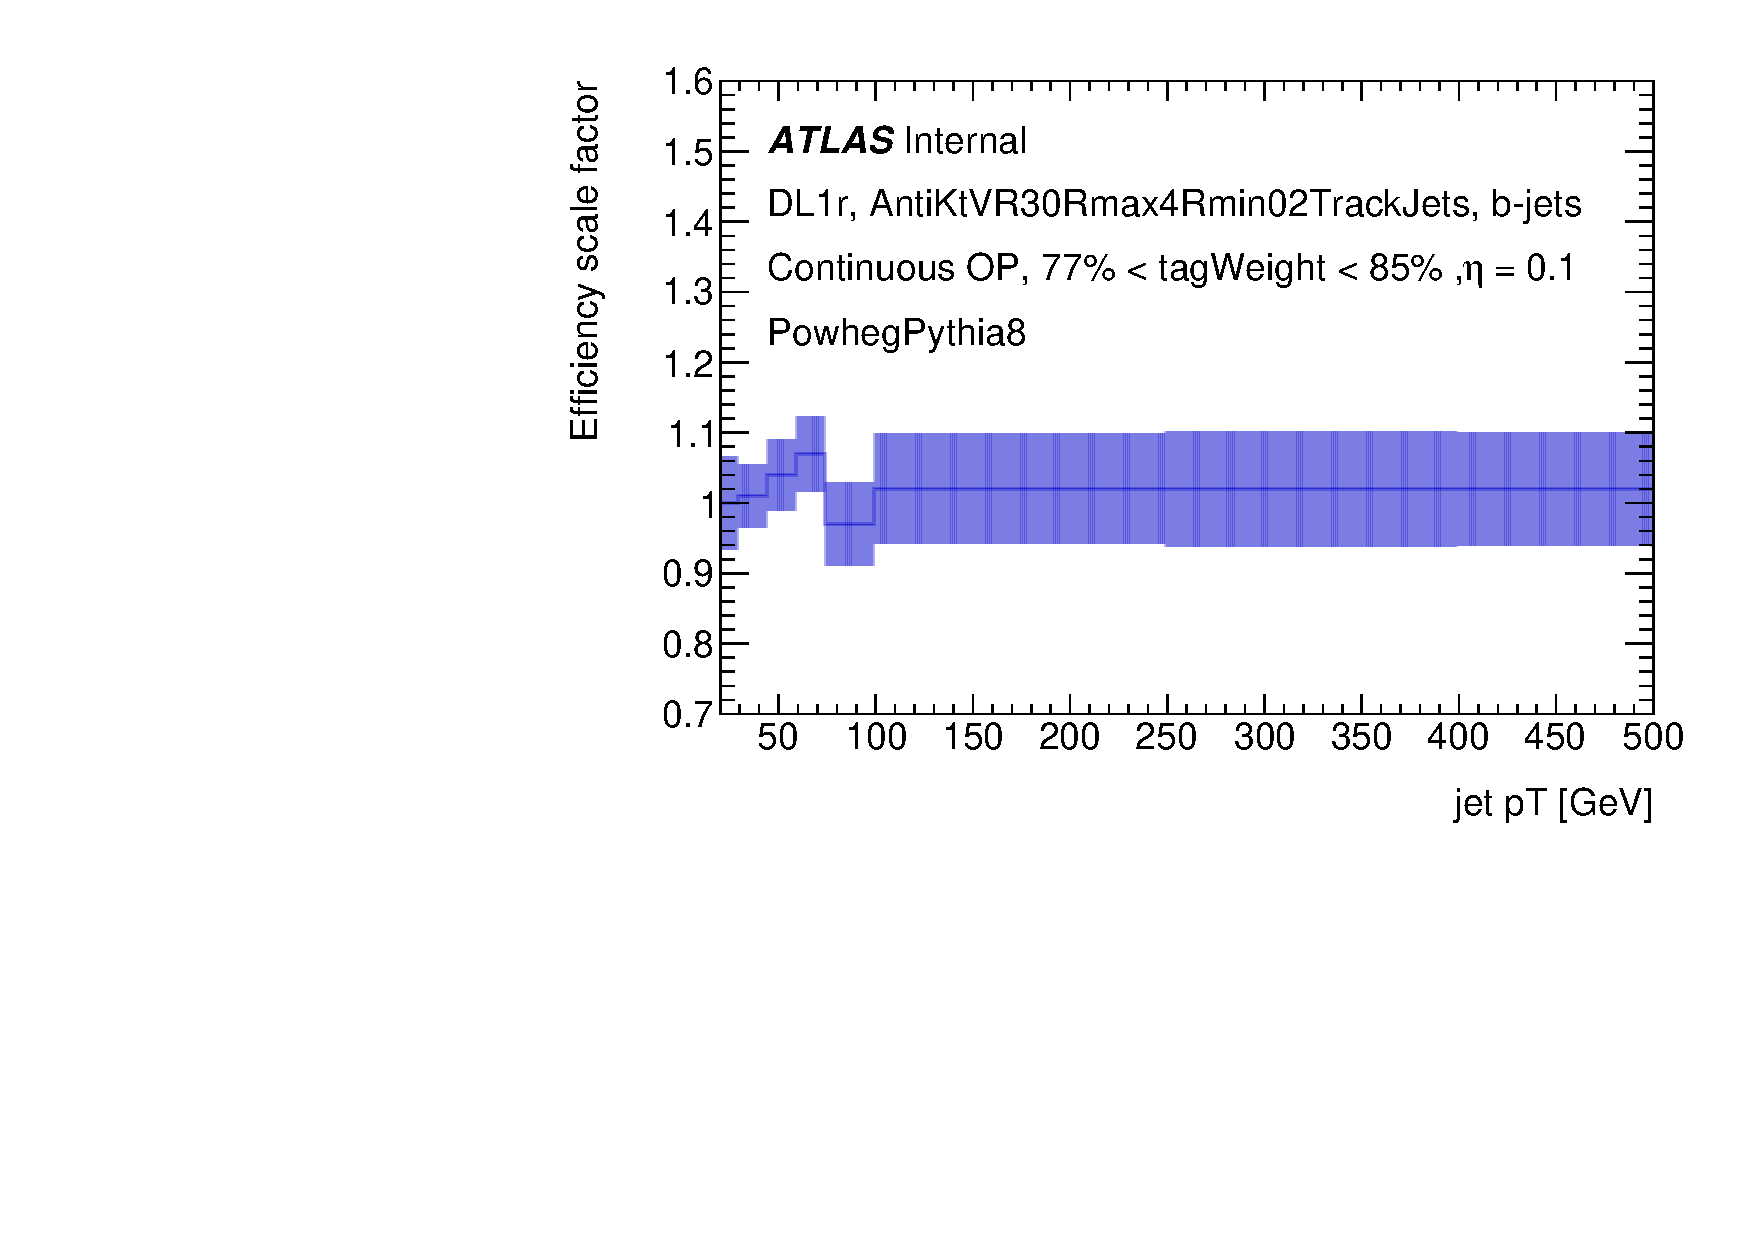
\includegraphics[width=0.4\linewidth]{Images/VH/Obj/FTAGCalib/ftagboo/DL1r_AntiKtVR30Rmax4Rmin02TrackJets_BTagging201903_Continuous_B_410470_77_85_eta01.pdf}}
         \subfigure{\label{subfig:FTAG_calibration_boosted_C}}{%
           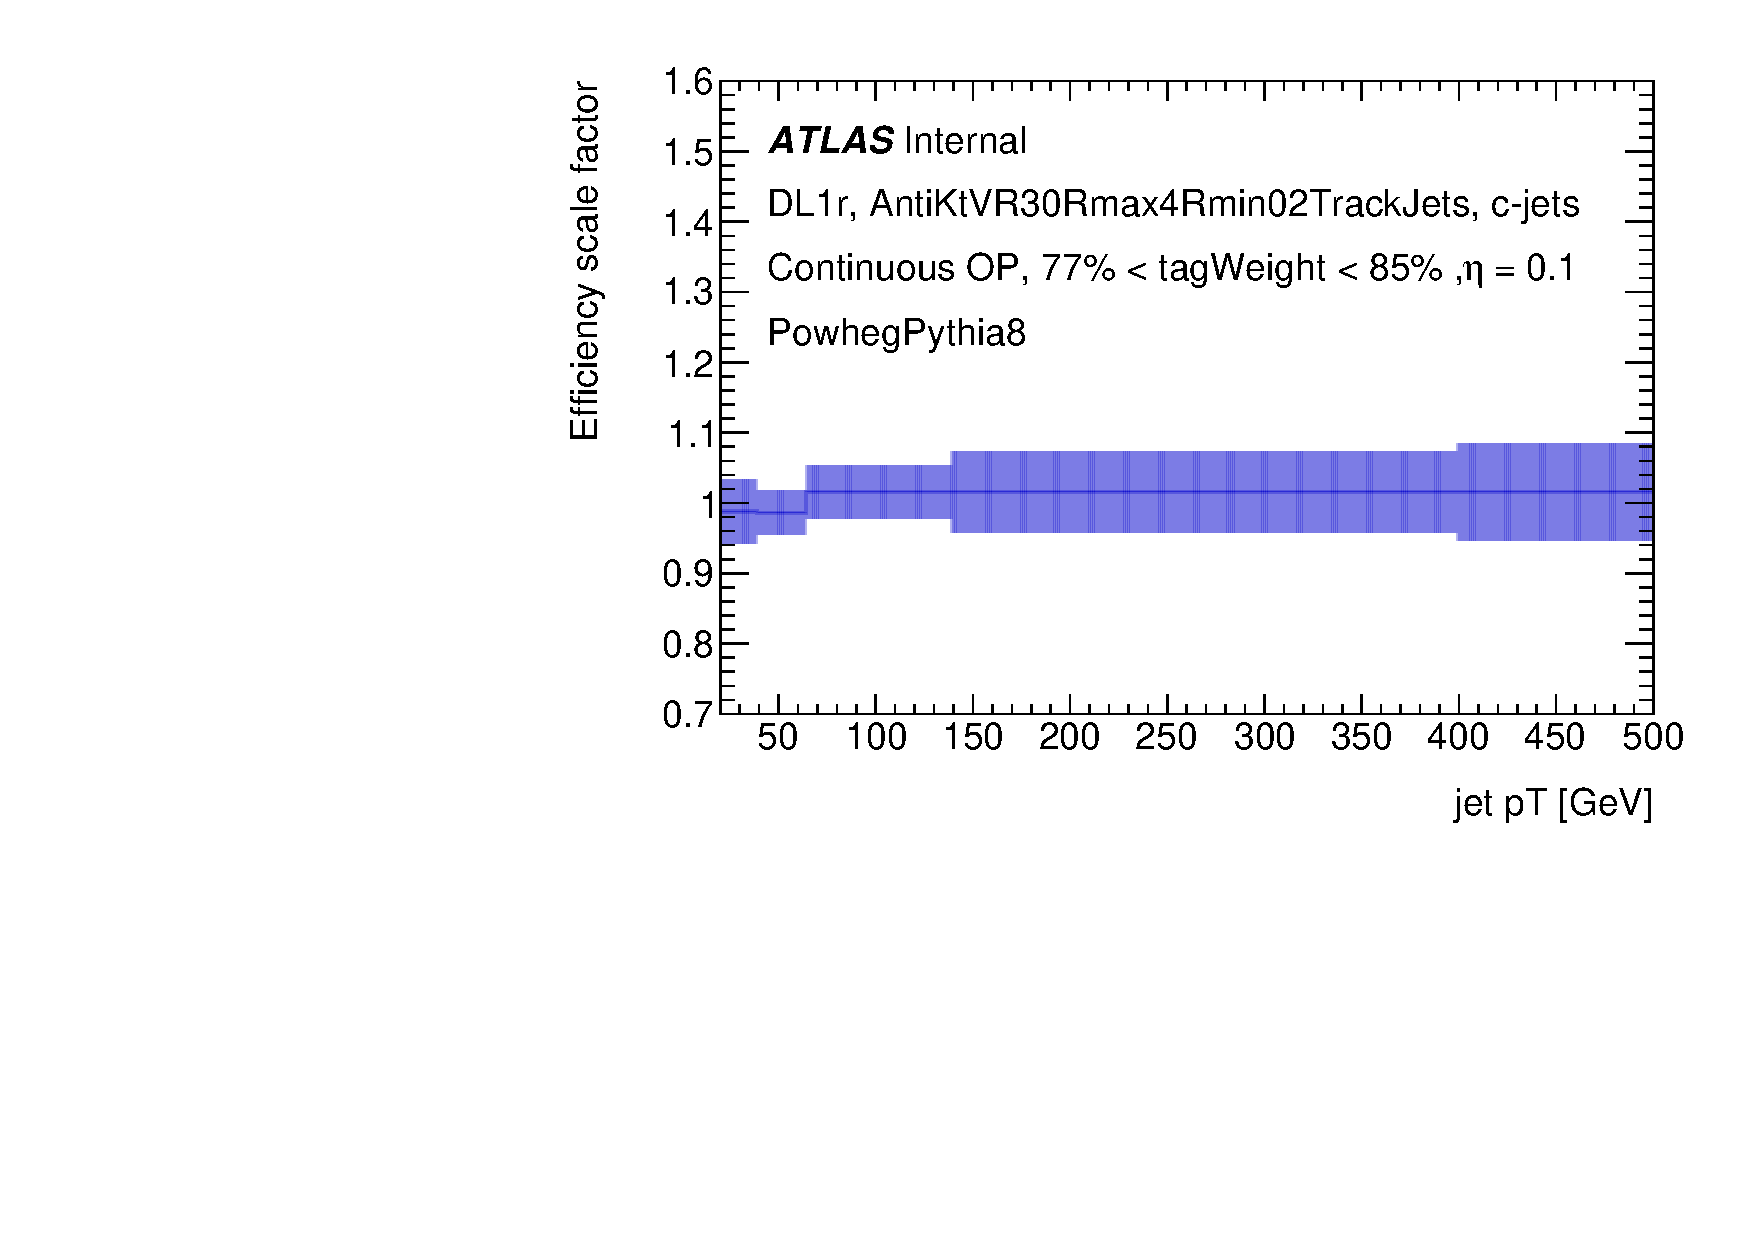
\includegraphics[width=0.4\linewidth]{Images/VH/Obj/FTAGCalib/ftagboo/DL1r_AntiKtVR30Rmax4Rmin02TrackJets_BTagging201903_Continuous_C_410470_77_85_eta01.pdf}} \\
         \subfigure{\label{subfig:FTAG_calibration_boosted_Light}}{%
           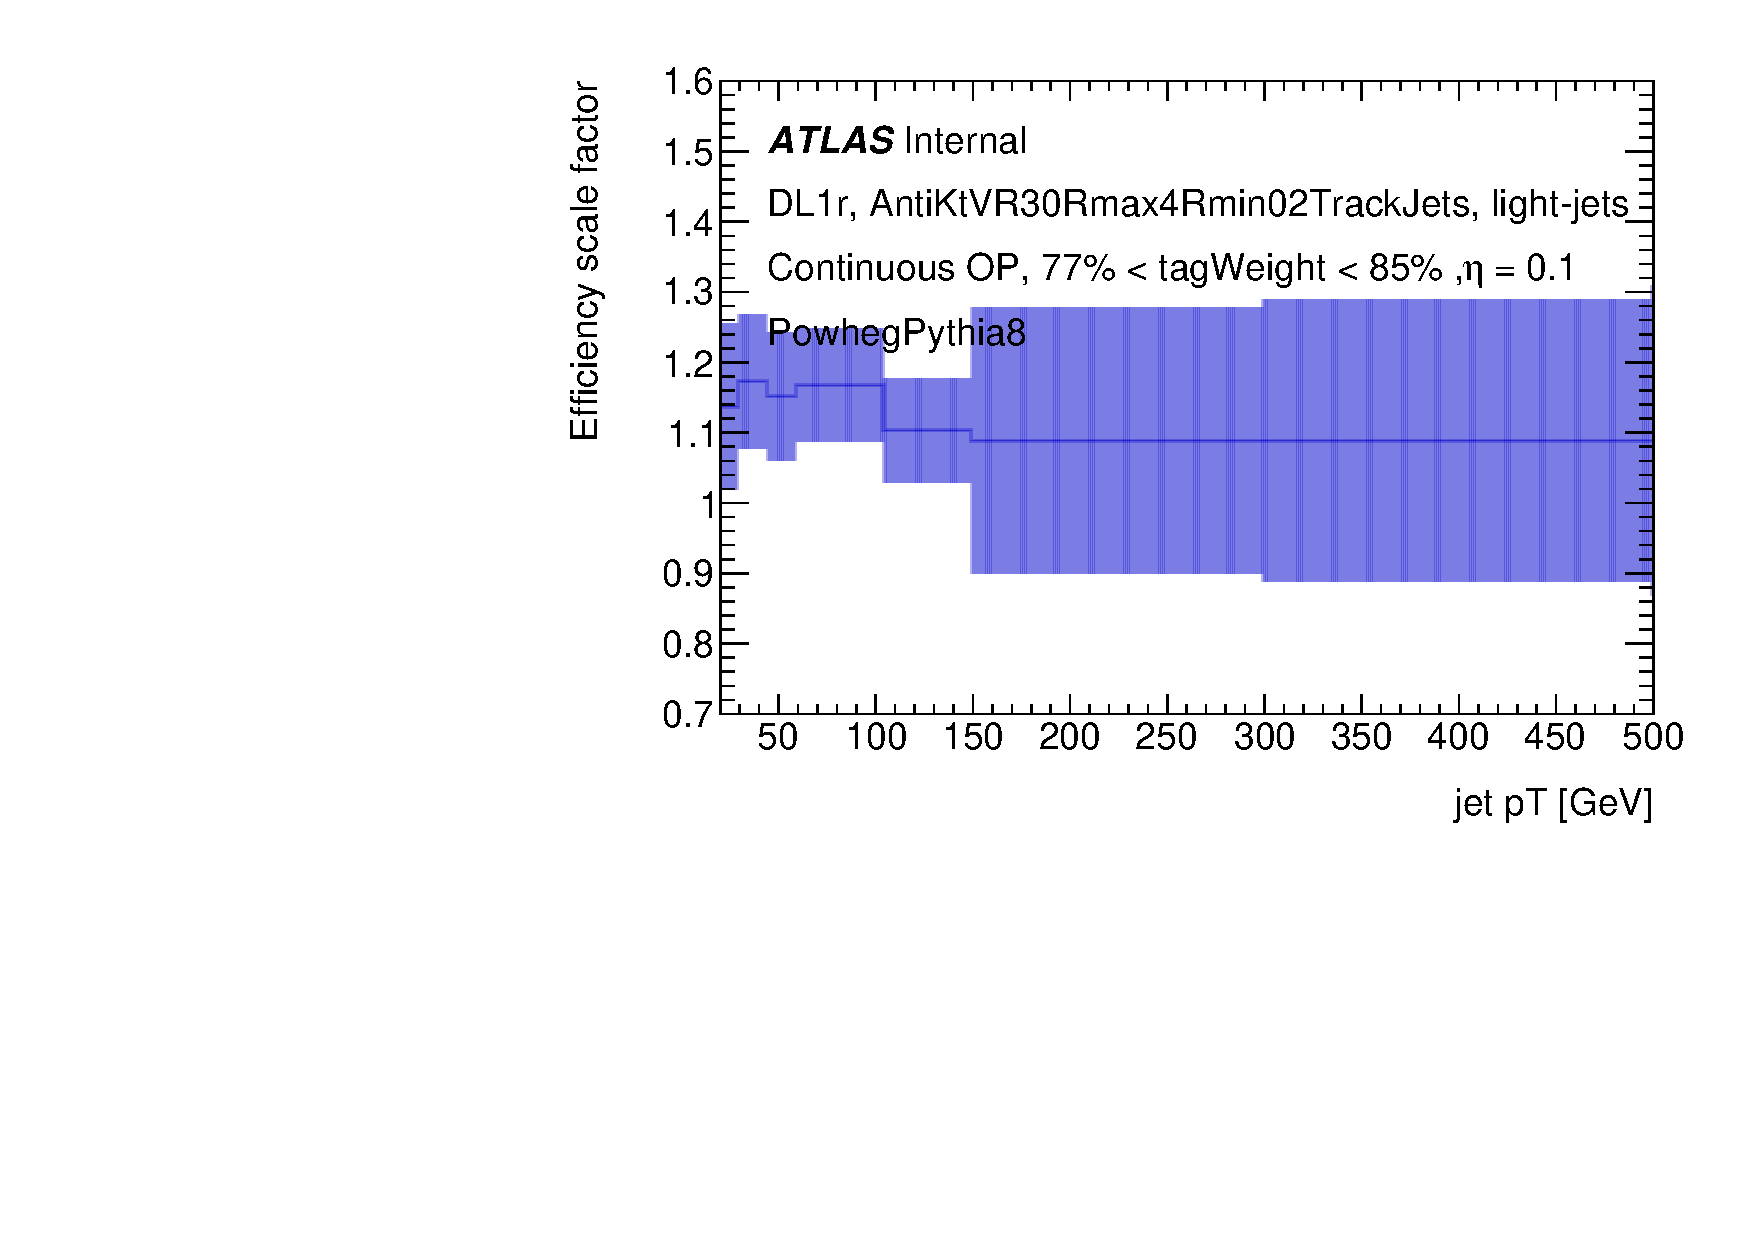
\includegraphics[width=0.4\linewidth]{Images/VH/Obj/FTAGCalib/ftagboo/DL1r_AntiKtVR30Rmax4Rmin02TrackJets_BTagging201903_Continuous_Light_410470_77_85_eta01.pdf}}
         \subfigure{\label{subfig:FTAG_calibration_boosted_T}}{%
           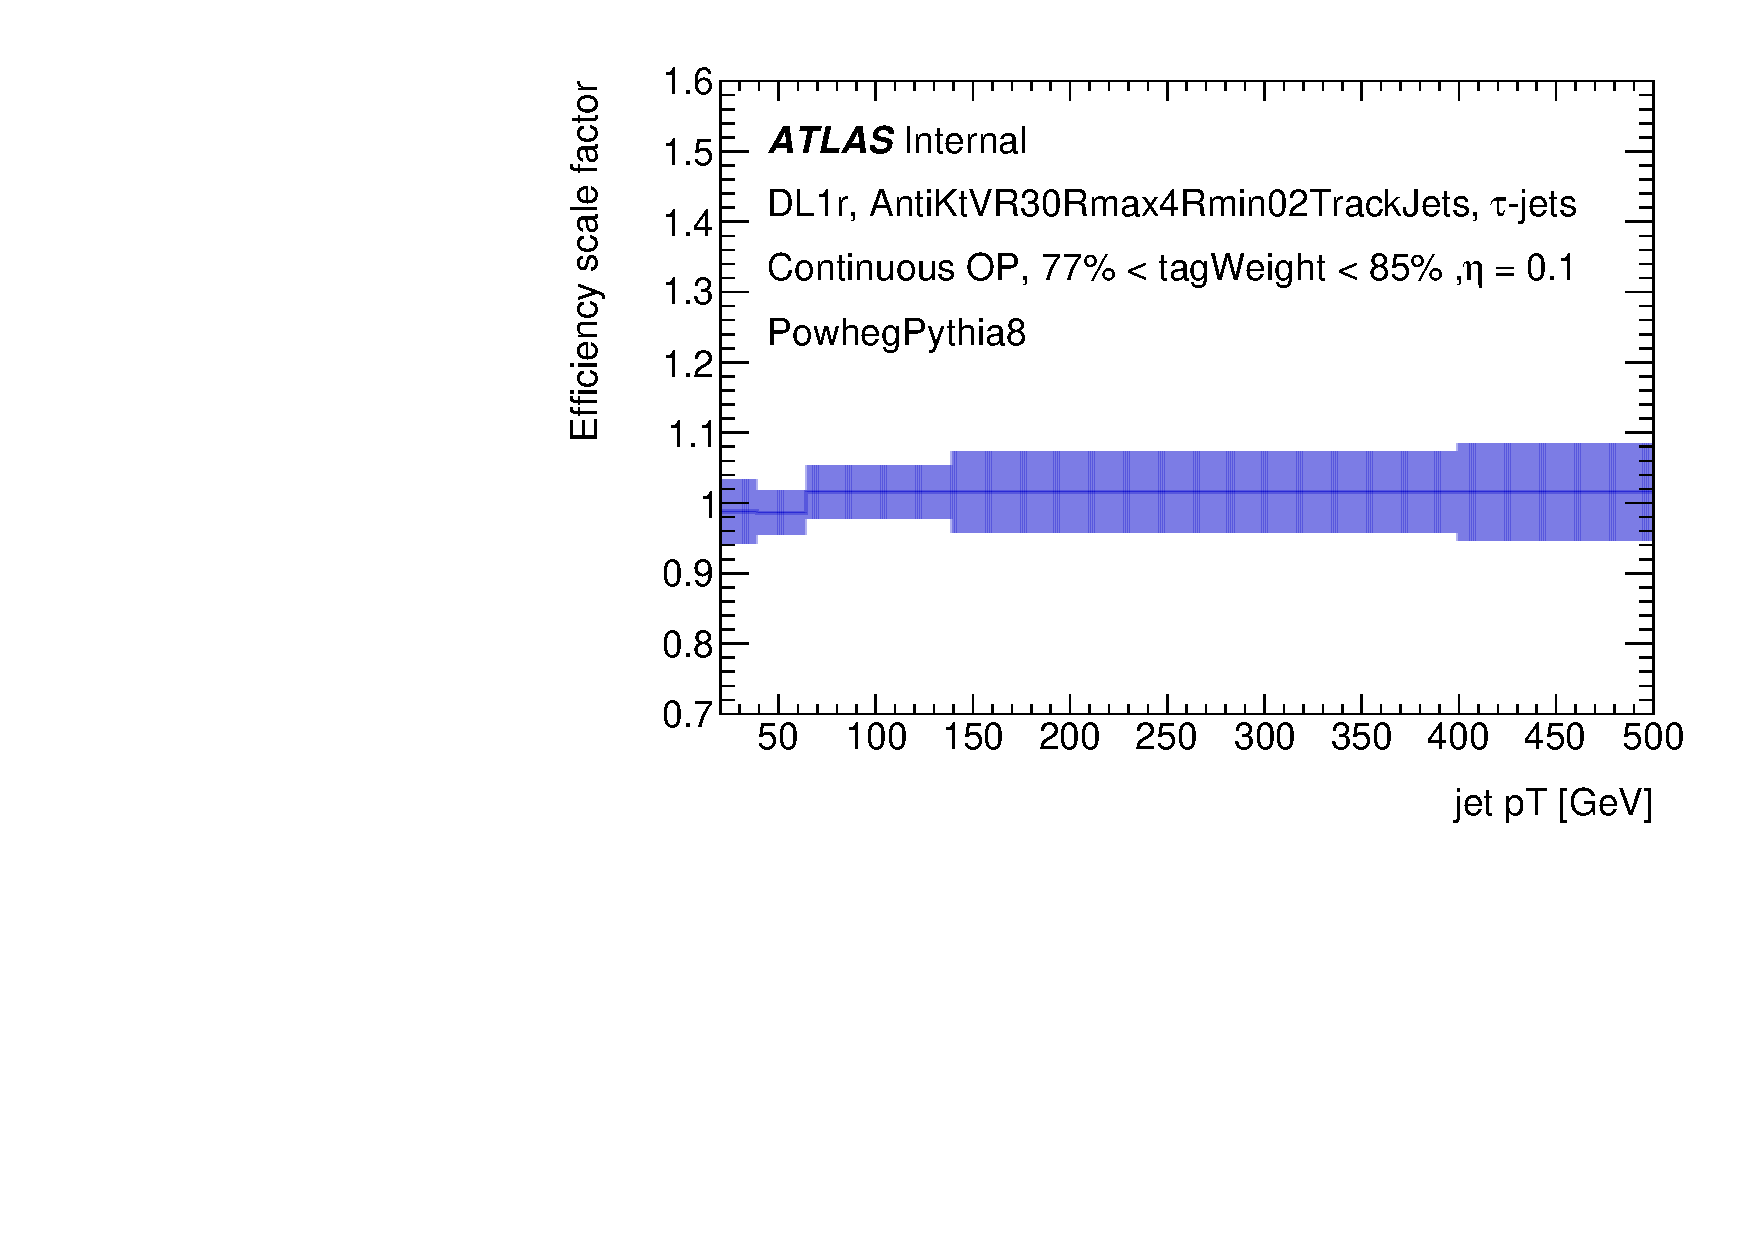
\includegraphics[width=0.4\linewidth]{Images/VH/Obj/FTAGCalib/ftagboo/DL1r_AntiKtVR30Rmax4Rmin02TrackJets_BTagging201903_Continuous_T_410470_77_85_eta01.pdf}}
       \caption{%
       Example of the boosted \vhb efficiency scale factor calibration results of the DL1r tagger on PowhegPythia8 \ttbar samples for the $77\%<\epsilon_j<85\%$ bin. The scale factors of $\tau$-jets are from $c$-jet calibration. From the internal documentation.
       }%
       \label{appfig:FTAG_calibration_boosted}
   \end{figure}
   

\section{Analysis Categorisation}\label{ap-vhCat}
This section offers more details in the categorisation of the $VH(H\rightarrow b\bar{b}/c\bar{c})$ Combined Analysis. The tagging requirements for an event to be in the \glsfirst{sr} are:
\begin{itemize}
\item For $VH(H\rightarrow b\bar{b})$, strictly two jets must be $b$-tagged and no tight $c$-tagged jets are allowed. 
\item For $VH(H\rightarrow c\bar{c})$, no $b$-tagged jets are allowed and at least one jet must be tight $c$-tagged. This defines three possible signal regions, where a second jet is either tight $c$-tagged ($TT$), loose $c$-tagged ($LT$), or not tagged ($TN$). 
\end{itemize}
Two control regions are defined by modifying the conditions on the tags of the jets in the event: 
\begin{itemize}
\item A combined $VH(H\rightarrow b\bar{b})$ and $VH(H\rightarrow c\bar{c})$ top control region (topCR) is obtained by requiring at least 1 $b$-tagged jet and 1 $c$-tagged jet. The definition of this control region is the core subject of this work and will be further addressed later in this report. 
\item For $VH(H\rightarrow c\bar{c})$ only, an additional control region is defined by requiring a loose $c$-tagged and a non $b$- nor $c$-tagged jets in the event to constrain the significant $V$+light-jet background. 
\end{itemize}

\subsection{The $\Delta R$ Cut Between Higgs Candidate Jets}\label{ap-sec-vh-deltaR}
The angular separation between the two candidate jets $\Delta R(j_1, j_2)$, as defined in Equation \ref{eq-deltaR}, can be used to define a control region enriched in $V$+jets and $t\bar{t}$ backgrounds since these two processes give candidate jets with a flat angular spectrum while the signal peaks at low values of $\Delta R$. A \textit{high $\Delta R$} control region (High $\Delta R$ CR) is defined using parametrised cuts on $\Delta R$ between the Higgs candidate jets as a function of $p_T^V$. An additional \textit{low $\Delta R$} control region (Low $\Delta R$ CR) for the 1L channel in the resolved \vhb is also introduced (for \vhc, it is merged with the signal region). The philosophy behind the parametrisation of this function is to adapt the cut on the expected angular separation between the two Higgs candidate jets as a function of how boosted they are, as described by the $p_T^V$ variable. For signal events, we expect the $H$ and $V$ to be approximately back-to-back hence $p_T^V$ is a good proxy for $p_T^H$ while benefiting from better experimental resolution, as it is reconstructed from leptons $p_T$ and/or $E_T$, depending on the channel. From physical principals, boosted candidate jets are indeed expected to have a lower angular separation. The cuts are defined by fitting a template function $ c_1 \times e^{c_2 + c_3 \times p_T^V}$ to the \vhb selected events, so that:   
\begin{itemize}
\item 95\% (85\%) of the \vhb signal is below the top limit for the 2-jet (3-jet) signal region,
\item 90\% of the diboson process is above the bottom limit in both signal regions.
\end{itemize}

The results of these fits for the 1L channel are displayed in Figure~\ref{fig:drccptvCutsVHcc}, showing the signal yield in a 2-dimensional histogram ($p_T^V$ vs $\Delta R_{c\bar{c}}$) for different tags applied. Cuts derived on the \vhc selected events showed good agreement with the \vhb derived cuts. The $VH(H\rightarrow b\bar{b})$ cuts is chosen so that the kinematic selection of the two analyses is harmonised. \\

\subsection{Resolved Top Control Region in 0L and 1L}
The top control region (topCR) is used to constrain the rather significant top background that peaks at signal-like values of the discriminant variables. Indeed, when the candidate jets selected correspond to the $b$- and $c$-jet from a $t\bar{t}$ decay, the invariant mass of the pair peaks at 120 GeV, exactly the region of interest for a Higgs decay search. The topCR is defined by requiring at least one $c$-tagged jet in combination with at least one $b$-tagged jet using the \textit{AllSignal} strategy, as previously described. This tagging requirement renders it orthogonal to the signal region of the analysis and targets the decay topology of the different top processes: 
\begin{itemize}
\item Semi-leptonic $t\bar{t}$ decay: both $t$ follow the usual decay chain  $t \rightarrow b$ + $W$, with one of the $W$ decaying leptonically and the other one to a pair of quarks. Some events from this process can enter the signal region when some of the quarks are $c$-tagged or if the $b$-jets are mis-tagged or flew out of the detector acceptance. Requiring the combination of a $b$-tag and a $c$-tag effectively selects this process, the $b$ coming from the direct $t$ decay and the $c$ from a subsequent $W$ decay. 
\item Single top $t$-quark: predominantly the $Wt$ process $W$ $t \rightarrow W$ +  $b$ + $W$, with one $W$ decaying leptonically and the other hadronically. Some of these background events can enter the signal region if the $b$- is missed and if a jet is $c$-tagged, from the extra $W$ or if the $b$-jet is mis-tagged. Events from the single-top $t$- and $s$-channel of the process $t \rightarrow b$ + $W$ bring a smaller contribution, as the $c$-tagged jet must come from \textit{Initial State Radiation} (ISR) or \textit{Final State Radiation} (FSR) if the $b$ is not mis-tagged. Single-top is a minor background in 0L and 1L, with the main component being the production of $Wt$ pairs. The $t$-channel and $s$-channel contribute less than 1\% of the total background.
\end{itemize}

Of the two processes, the $t\bar{t}$ is therefore the most important one and a main background in the 0L and 1L channels. Due to their similarities, the $t\bar{t}$ and $Wt$ processes are considered as a single \textit{top} background in the analysis. In 2L, because this top background is small, no flavour-based topCRs are introduced and a different strategy is employed where the top is directly constrained in a pure top-$e\mu$ control region defined by requiring two charged leptons of different flavours. For the 0L and 1L channels, the expected top background normalisation and its kinematic distributions, as given by the MC simulation, are adjusted using data in the topCRs; this is extrapolated to the signal regions under consideration of extrapolation effects (and corresponding extrapolation uncertainties) that account for differences between the topCRs and SRs. \\

The combined top background is separated into different components, depending on the true flavour of the two candidate jets, that can be combined during the statistical analysis. These are:
\begin{itemize}
\item top($bb$): in this case, the two $b$-jets produced during the $t\bar{t}$ decay are selected. This is a small component in the signal regions of the $VH(H\rightarrow c\bar{c})$ analysis, due to the 70\% efficiency WP for $b$-tagging and the low mis-tag rate for $b$-jets in $c$-tagging. Naturally, in $VH(H\rightarrow b\bar{b})$ it is the leading contribution. Due to the origin of the candidate jets, a large $\Delta R_{b\bar{b}}$ is expected between the two $b$-jets so this component is most effectively constrained by the High $\Delta R$ CR. 
\item top($bc$): where the $b$ is from a $t$ decay and the $c$ from a subsequent $W$ hadronic decay (or from ISR/FSR though this is less likely). Given the definition of the topCR, this is the dominating component in that region and the most important to constrain in the signal regions of the $VH(H\rightarrow b\bar{b}/c\bar{c})$ analyses due to its signal-like kinematics. 
\item top($bl$): where $l$ stands for anything not $b$ nor $c$ (light jets predominantly but also some mis-tagged hadronic $\tau$). This component is similar to the top($bc$) as it also consists of a $b$ + a jet from the $W$ and can end up in the SRs and topCRs due to mis-tags.
\item top($lq$): where $l$ is as above and $q$ can be any sort of jet except a $b$. This is a small component that mostly accumulates in the background-like part of the BDT score distribution. It is not constrained in the high $\Delta R$ regions nor the topCRs.
\end{itemize}
The signal region distributions in the 1L channel in the $p_T^V$ range $[150, 250]$ GeV are displayed in Figure~\ref{fig:SRslowptv}. While the top is not the dominant background, except in the tighter tagged TT 3-jet region, its relative contribution to the background composition increases at signal-like values of the discriminant, as shown in Figure~\ref{fig:topContentSR}. \\

\begin{figure}[h!]
%\hspace{-2.0cm}
\center
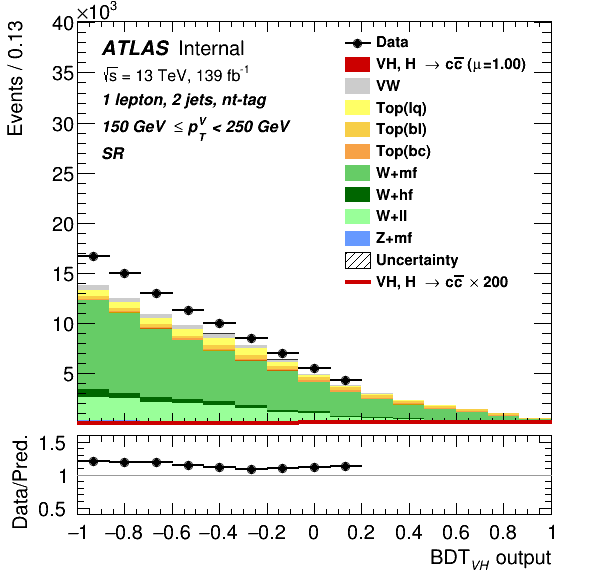
\includegraphics[width=0.32\textwidth]{Images/VH/SRsandTopCRs/Region_distmva_DSR_BMax250_L1_Y6051_TTypent_T1_J2_BMin150_Prefit.png}
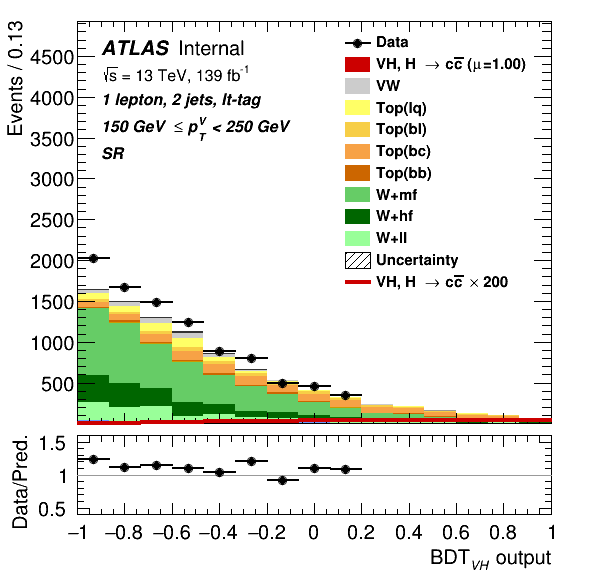
\includegraphics[width=0.32\textwidth]{Images/VH/SRsandTopCRs/Region_distmva_DSR_BMax250_L1_Y6051_TTypelt_T2_J2_BMin150_Prefit.png}
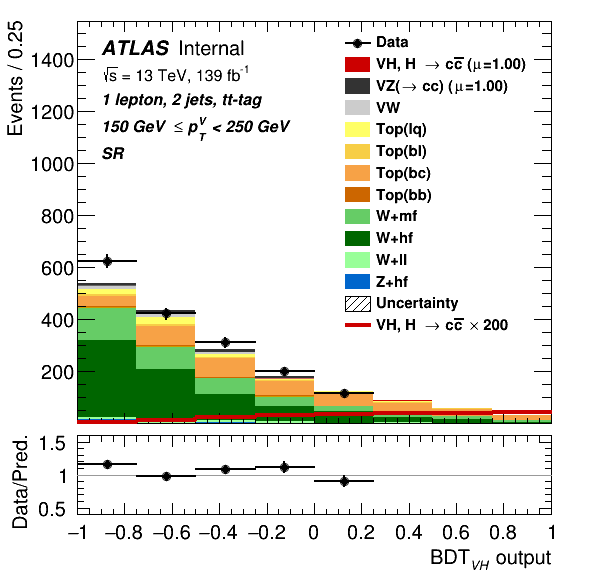
\includegraphics[width=0.32\textwidth]{Images/VH/SRsandTopCRs/Region_distmva_DSR_BMax250_L1_Y6051_TTypett_T2_J2_BMin150_Prefit.png}\\
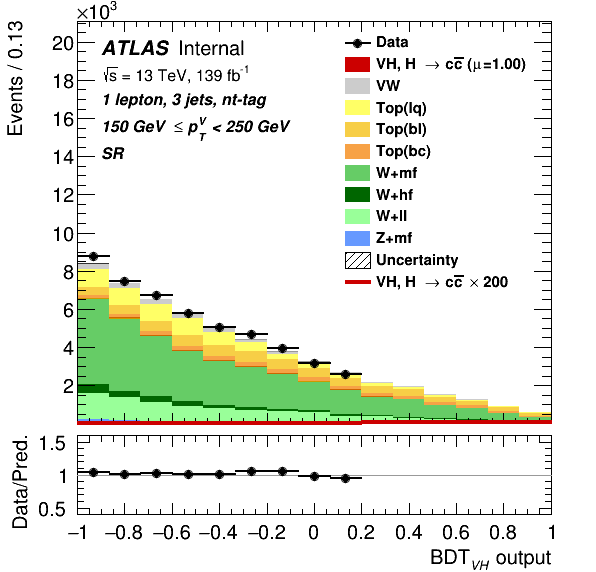
\includegraphics[width=0.32\textwidth]{Images/VH/SRsandTopCRs/Region_distmva_DSR_BMax250_L1_Y6051_TTypent_T1_J3_BMin150_Prefit.png}
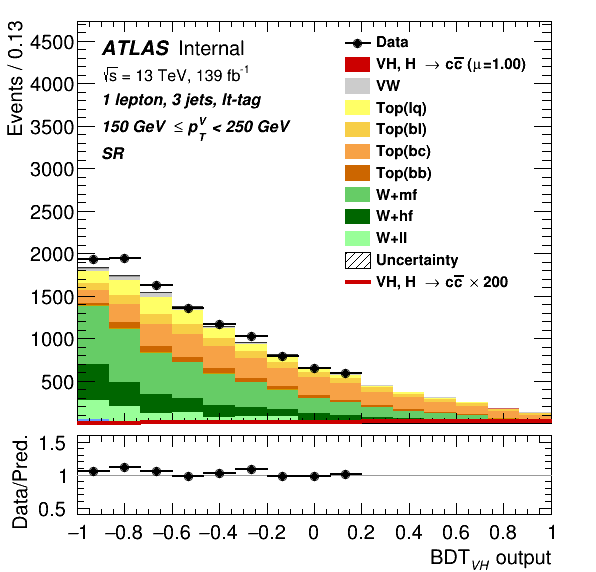
\includegraphics[width=0.32\textwidth]{Images/VH/SRsandTopCRs/Region_distmva_DSR_BMax250_L1_Y6051_TTypelt_T2_J3_BMin150_Prefit.png}
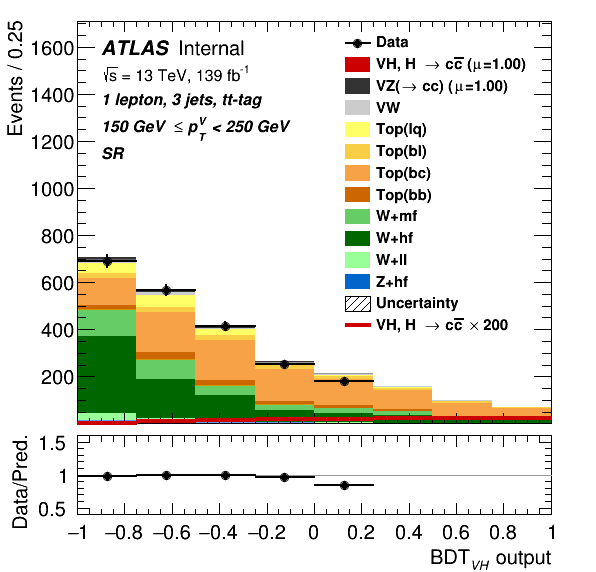
\includegraphics[width=0.32\textwidth]{Images/VH/SRsandTopCRs/Region_distmva_DSR_BMax250_L1_Y6051_TTypett_T2_J3_BMin150_Prefit.png}
\caption{The 1L signal regions BDT distributions in the low [150-250] $p_T^V$ range. Left: NT; centre: LT; right: TT. Top: 2 jets; bottom: 3 jets.} 
\label{fig:SRslowptv}
\end{figure}

The components contributing the most in the $VH(H\rightarrow c\bar{c})$ side of the analysis are the top($bc$) and top($bl$), due to the tagging requirement. There is very little top($bb$) thanks to the good performance of the tagger. Top($lq$) is mostly found in the looser tag regions (NT, LT) and not where the signal peaks. Figure~\ref{fig:topCRslowptv} displays the new top control regions proposed in this work: as expected, the bulk of the distributions is made of top background, centred around the expected Higgs mass. The philosophy behind the proposed new design leverages the pseudo-continuous tagging to select the highest $p_T$ $b$-tagged and $c$-tagged jets as Higgs candidates. Thus, BL and BT regions are defined depending on whether the highest $p_T$ $c$-tagged jet is loose- or tight-tagged. The regions are further split in the number of jets and the same definition is used in the 0L channel. The full tag compositions of each region are as follows:

\begin{itemize}
\item 2-jet: \quad BL: $BL$;  \quad BT: $BT$
\item 3-jet:  \quad BL: $BLN$, $BLL$;  \quad BT: $BTN$, $BTL$, $BTT$, and $BBT$
\end{itemize}
In the \textit{AllSignal} strategy, the Higgs candidates in the topCR are always the highest $p_T$ $b$- and $c$-tagged jets. This selection was observed to make the top control region distributions more closely match the distributions in the signal regions. \\

\begin{figure}[h!]
\center
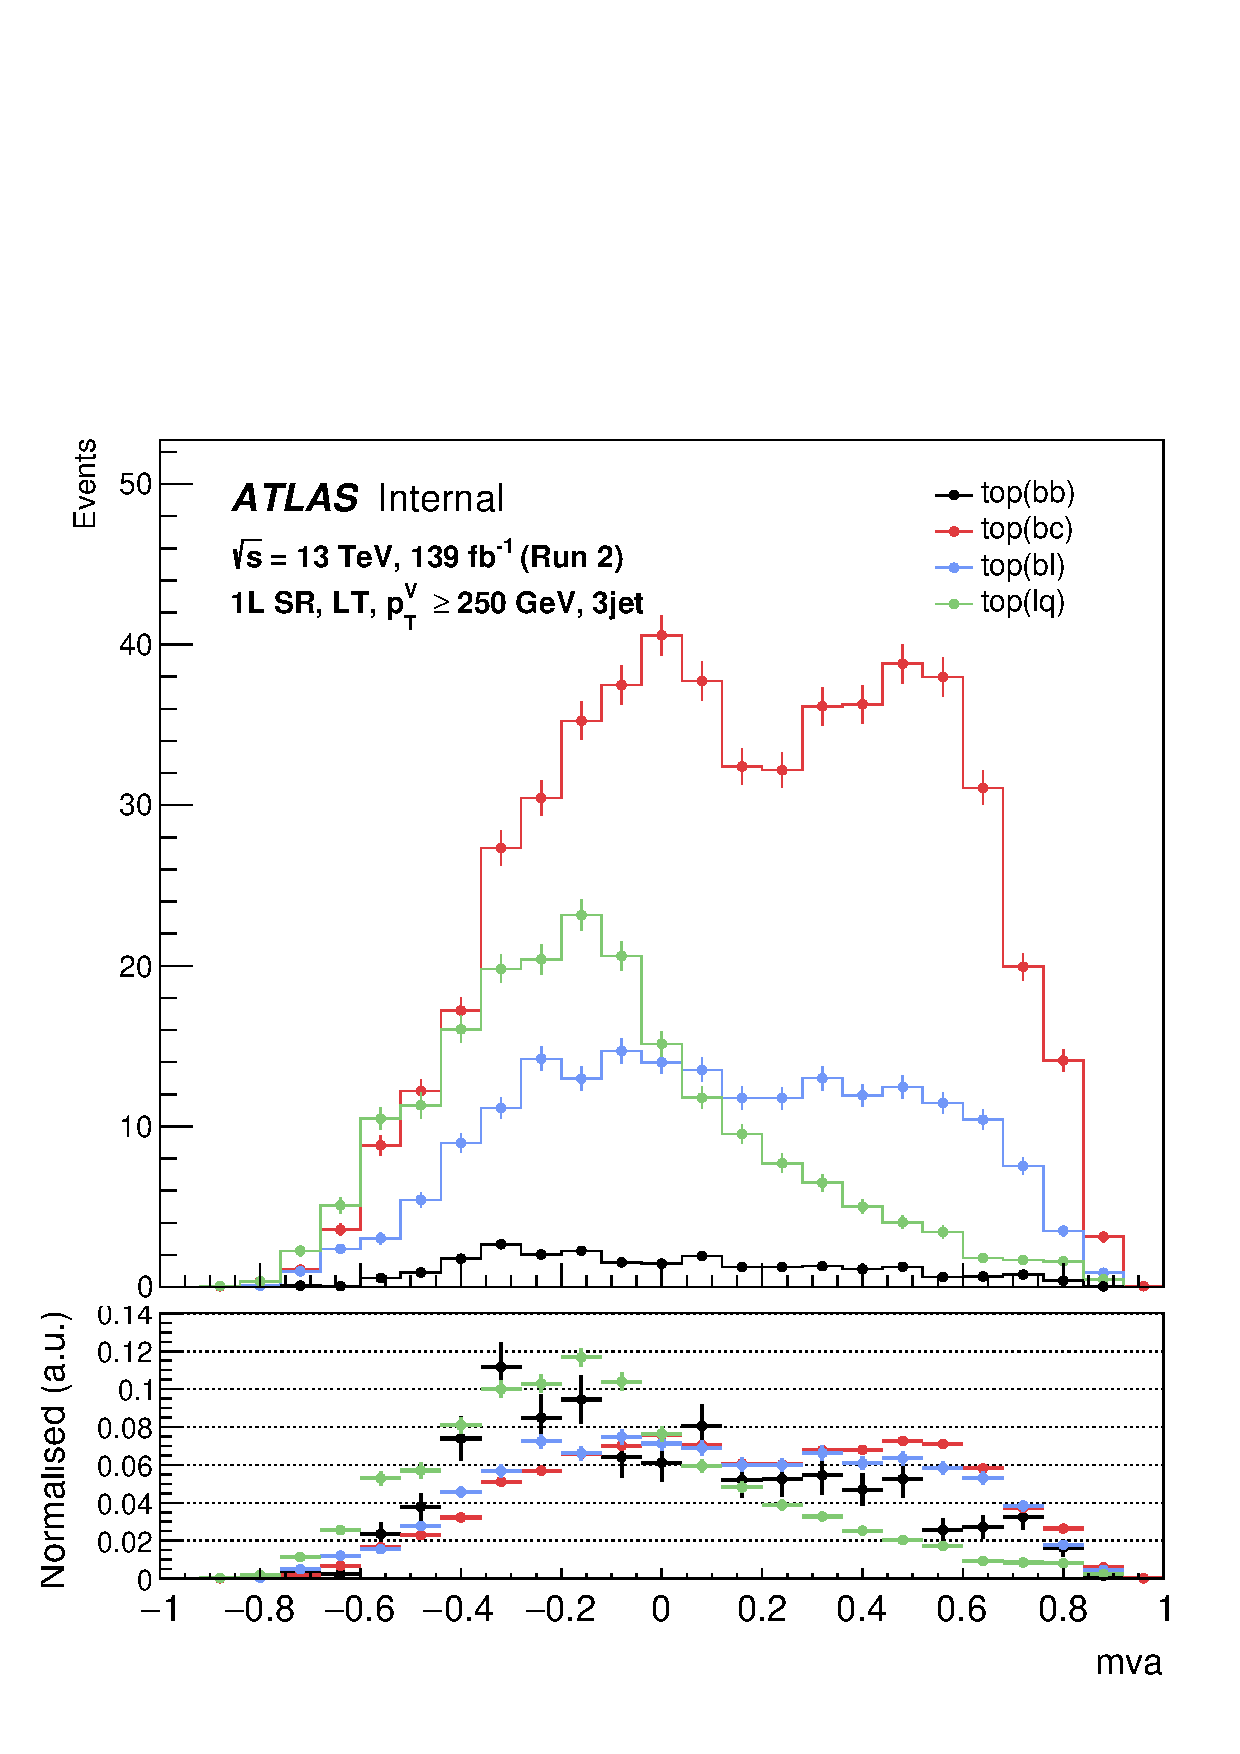
\includegraphics[width=0.48\textwidth]{Images/VH/top/OneLepton_top_2lttag3jet_SR_250ptv_mva.pdf}
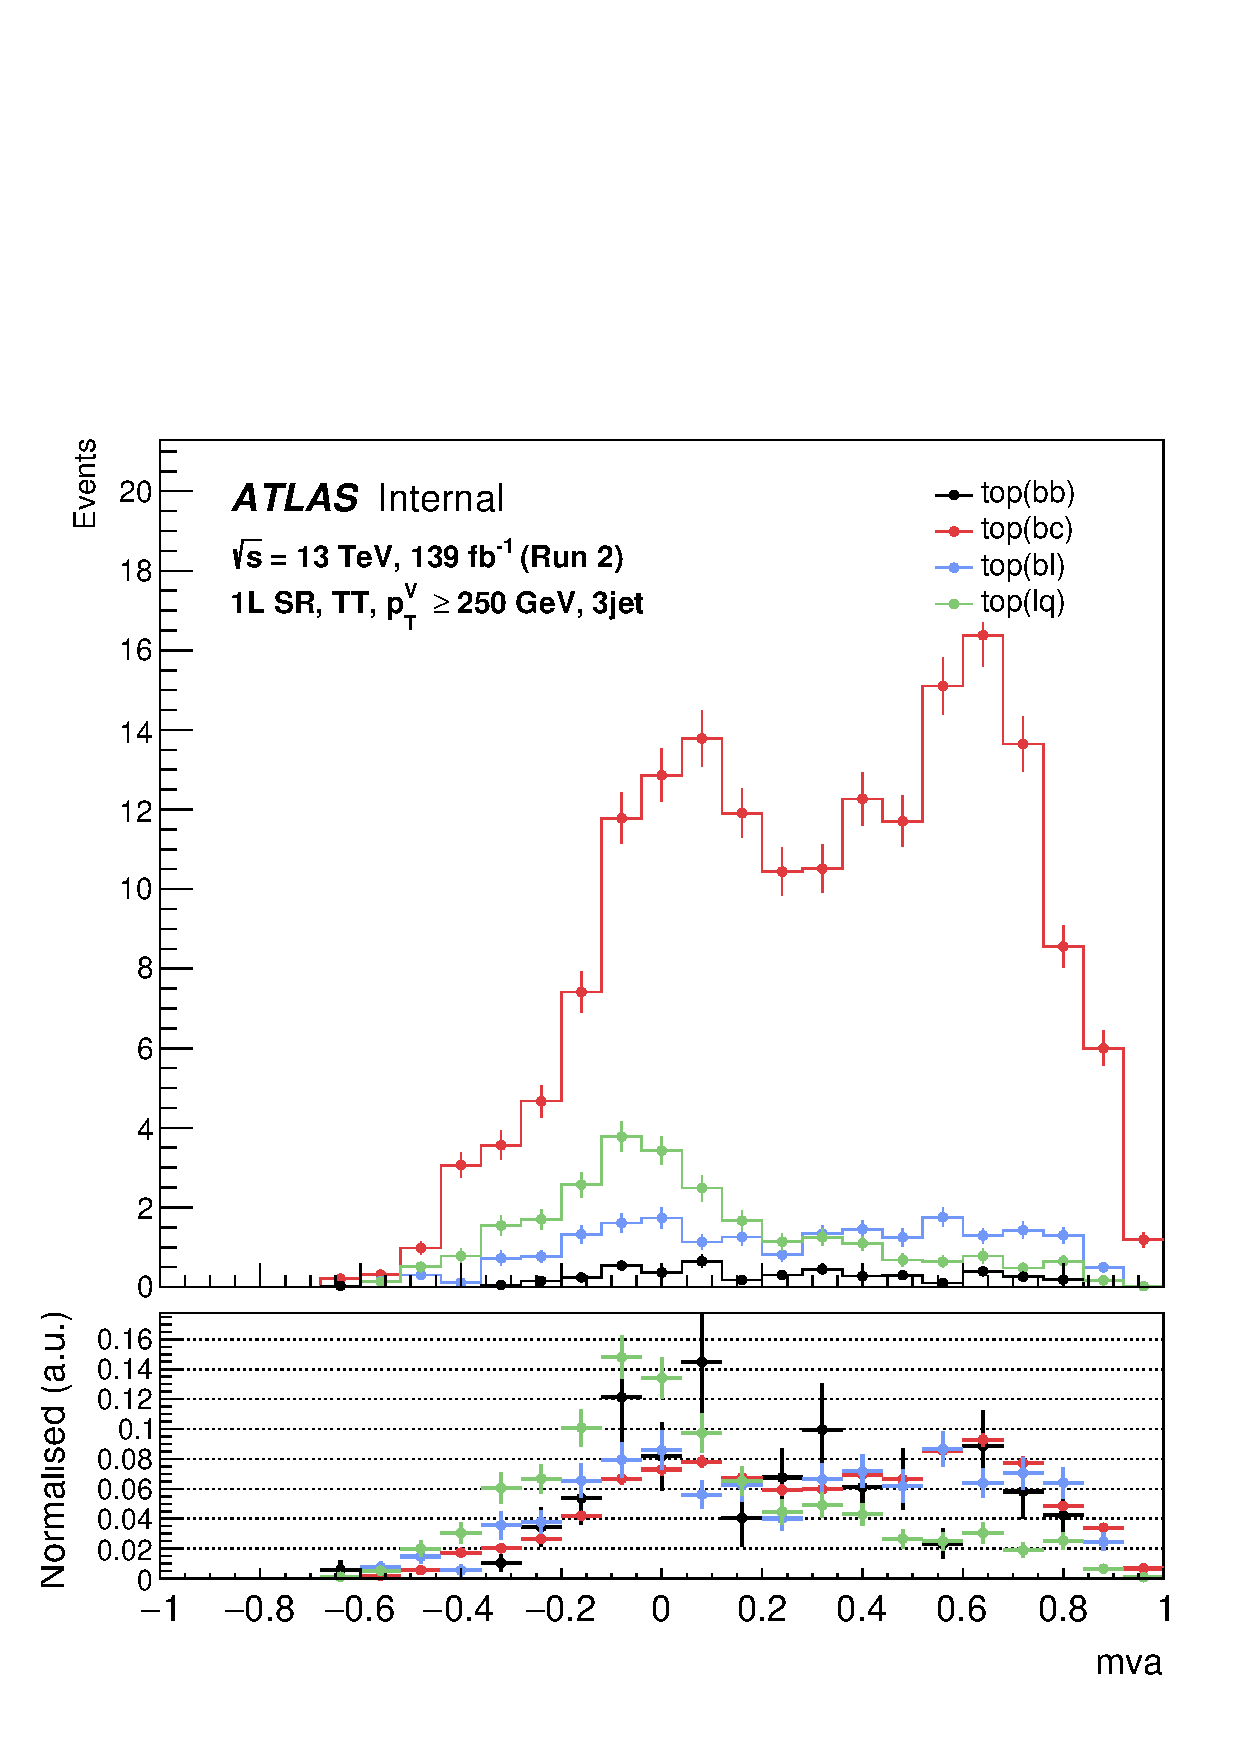
\includegraphics[width=0.48\textwidth]{Images/VH/top/OneLepton_top_2tttag3jet_SR_250ptv_mva.pdf}
\caption{Top components in the 1L 3 jets signal regions BDT distributions in the $\geq$ 250 GeV $p_T^V$ range. Left: LT; right: TT.}
\label{fig:topContentSR}
\end{figure}

\begin{figure}[h!]
%\hspace{-2.0cm}
\center
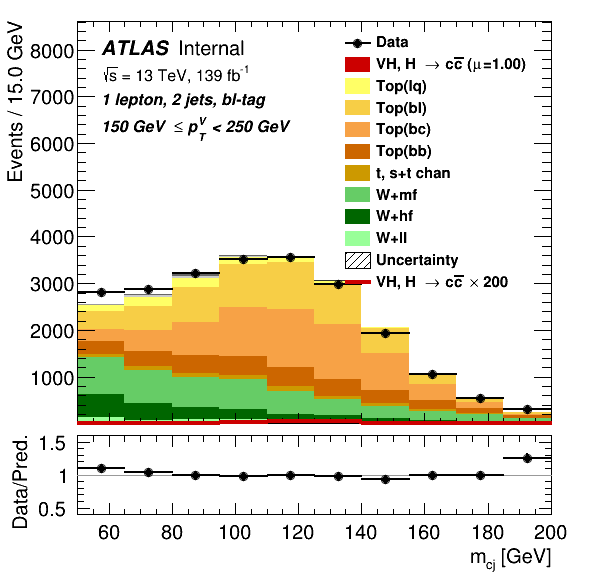
\includegraphics[width=0.24\textwidth]{Images/VH/SRsandTopCRs/Region_distmBB_DtopCRBL_BMax250_L1_Y6051_TTypebl_T1_J2_BMin150_Prefit.png}
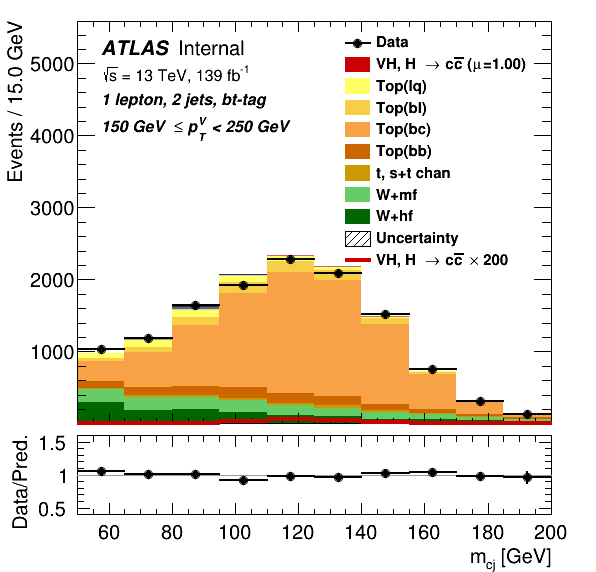
\includegraphics[width=0.24\textwidth]{Images/VH/SRsandTopCRs/Region_distmBB_DtopCRBC_BMax250_L1_Y6051_TTypebt_T1_J2_BMin150_Prefit.png}
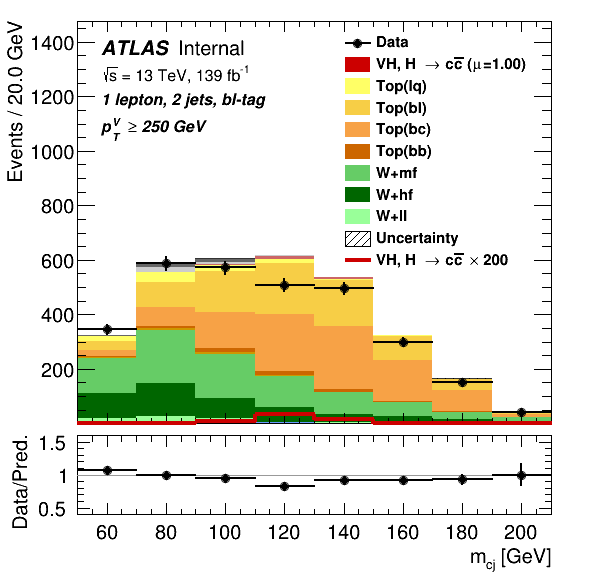
\includegraphics[width=0.24\textwidth]{Images/VH/SRsandTopCRs/Region_distmBB_DtopCRBL_L1_Y6051_TTypebl_T1_J2_BMin250_Prefit.png}
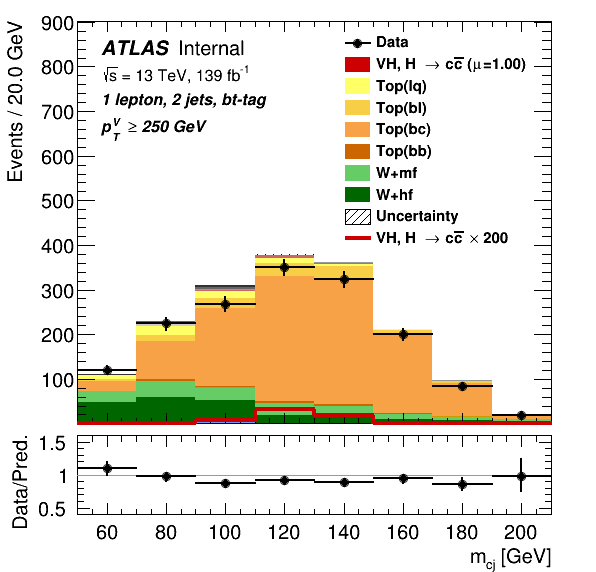
\includegraphics[width=0.24\textwidth]{Images/VH/SRsandTopCRs/Region_distmBB_DtopCRBC_L1_Y6051_TTypebt_T1_J2_BMin250_Prefit.png}\\

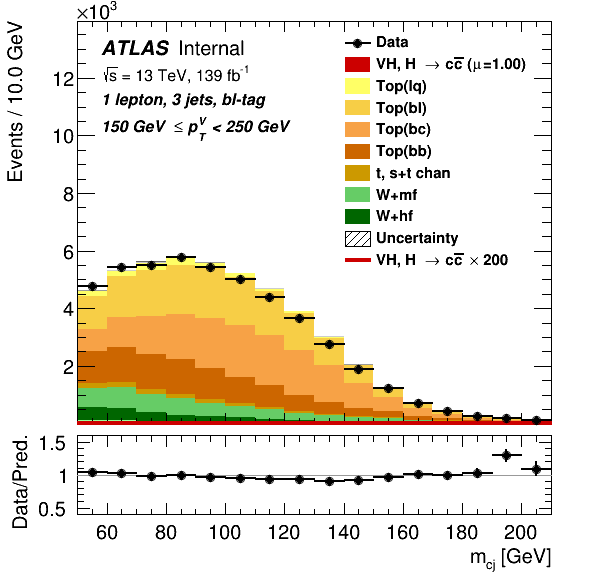
\includegraphics[width=0.24\textwidth]{Images/VH/SRsandTopCRs/Region_distmBB_DtopCRBL_BMax250_L1_Y6051_TTypebl_T1_J3_BMin150_Prefit.png}
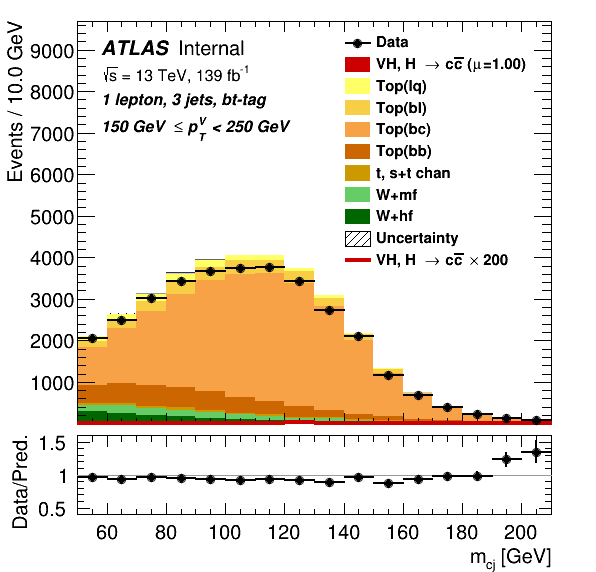
\includegraphics[width=0.24\textwidth]{Images/VH/SRsandTopCRs/Region_distmBB_DtopCRBC_BMax250_L1_Y6051_TTypebt_T1_J3_BMin150_Prefit.png}
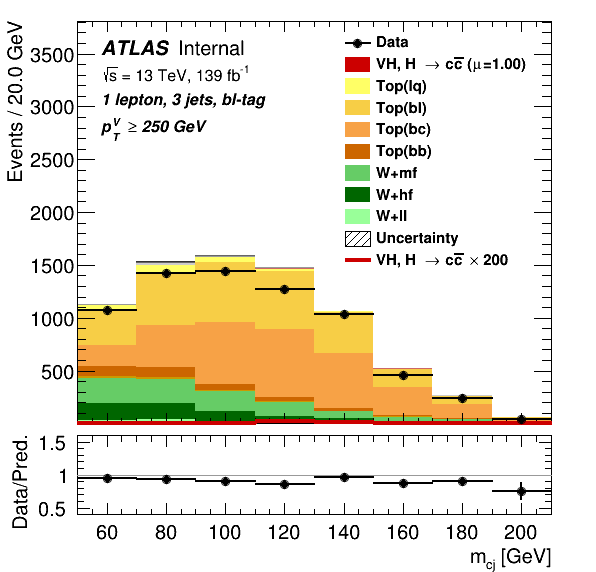
\includegraphics[width=0.24\textwidth]{Images/VH/SRsandTopCRs/Region_distmBB_DtopCRBL_L1_Y6051_TTypebl_T1_J3_BMin250_Prefit.png}
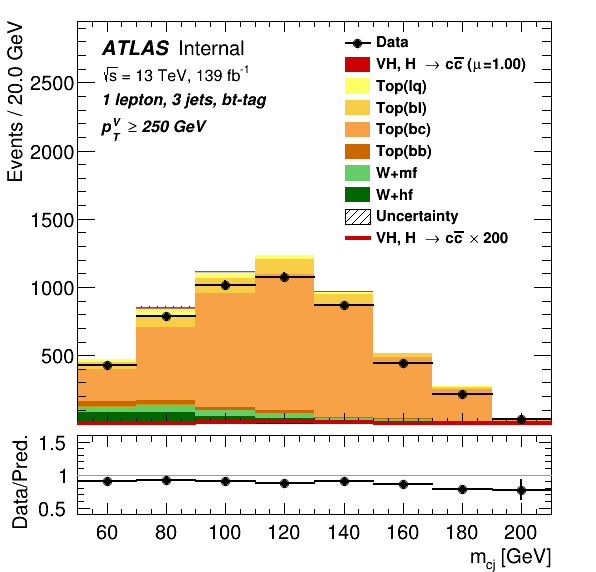
\includegraphics[width=0.24\textwidth]{Images/VH/SRsandTopCRs/Region_distmBB_DtopCRBC_L1_Y6051_TTypebt_T1_J3_BMin250_Prefit.png}
\caption{The 1L top control regions $m_{c\bar{c}}$ distributions in both $p_T^V$ ranges (left two columns are [150, 250] GeV, right two are > 250 GeV). Per group of two adjacent: left is BL, right is BT. Top: 2 jets; bottom: 3 jets.} 
\label{fig:topCRslowptv}
\end{figure}

\begin{figure}[h!]
\center
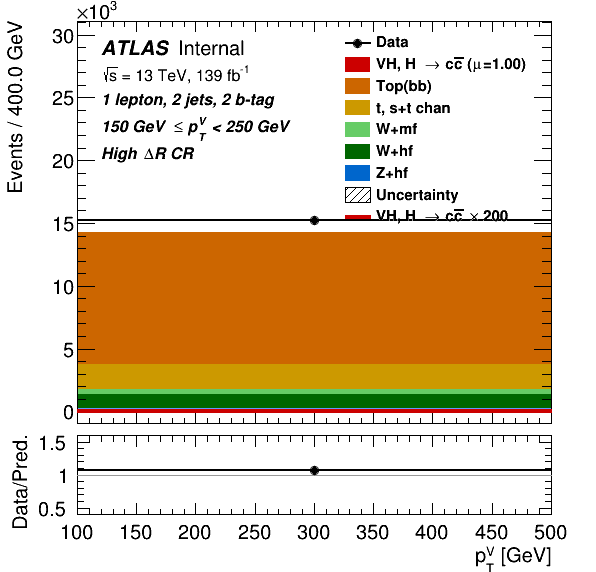
\includegraphics[width=0.48\textwidth]{Images/VH/SRsandTopCRs/Region_distpTV_DCRHigh_BMax250_L1_Y6051_TTypebb_T2_J2_BMin150_Prefit.png}
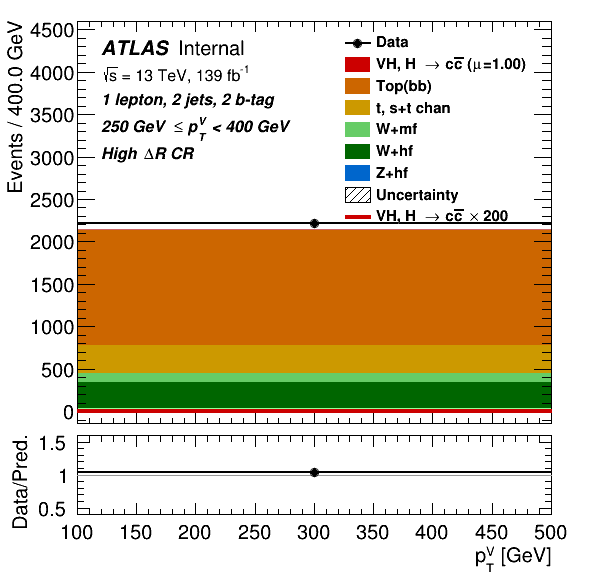
\includegraphics[width=0.48\textwidth]{Images/VH/SRsandTopCRs/Region_distpTV_DCRHigh_BMax400_L1_Y6051_TTypebb_T2_J2_BMin250_Prefit.png}\\
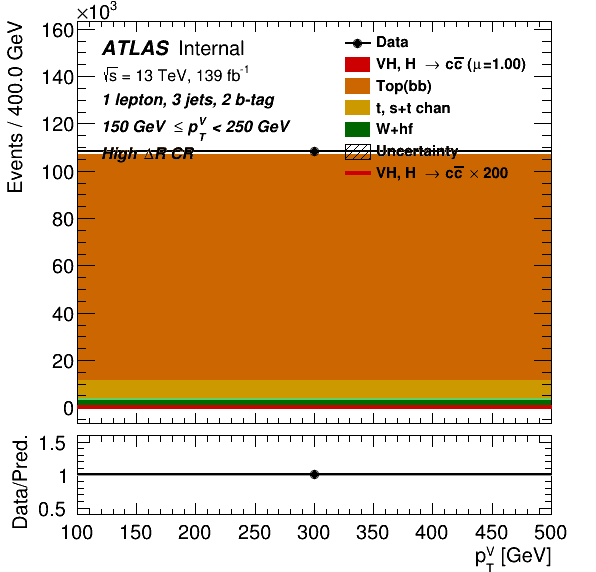
\includegraphics[width=0.48\textwidth]{Images/VH/SRsandTopCRs/Region_distpTV_DCRHigh_BMax250_L1_Y6051_TTypebb_T2_J3_BMin150_Prefit.png}
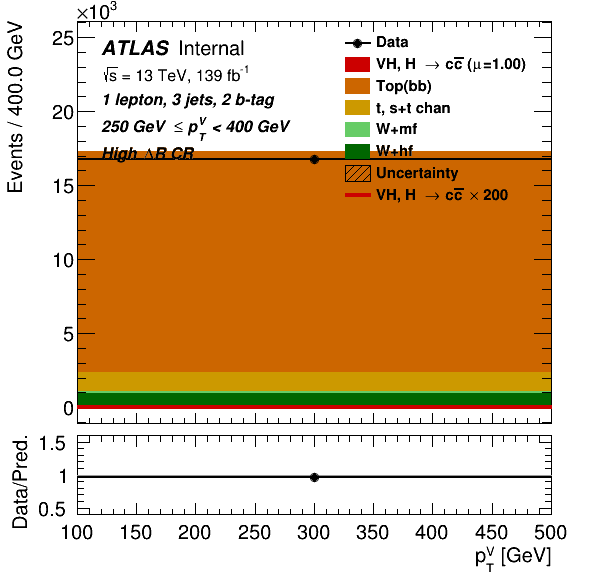
\includegraphics[width=0.48\textwidth]{Images/VH/SRsandTopCRs/Region_distpTV_DCRHigh_BMax400_L1_Y6051_TTypebb_T2_J3_BMin250_Prefit.png}
\caption{The 1L 1-bin  $VH(H\rightarrow b\bar{b})$ High $\Delta R$ CR in both $p_T^V$ ranges. Left: [150, 250] GeV; right: [250, 400] GeV. Top: 2 jets; bottom: 3 jets.} 
\label{fig:vhbbDRCR}
\end{figure}

\begin{figure}[h!]
%\hspace{-2.0cm}
\center
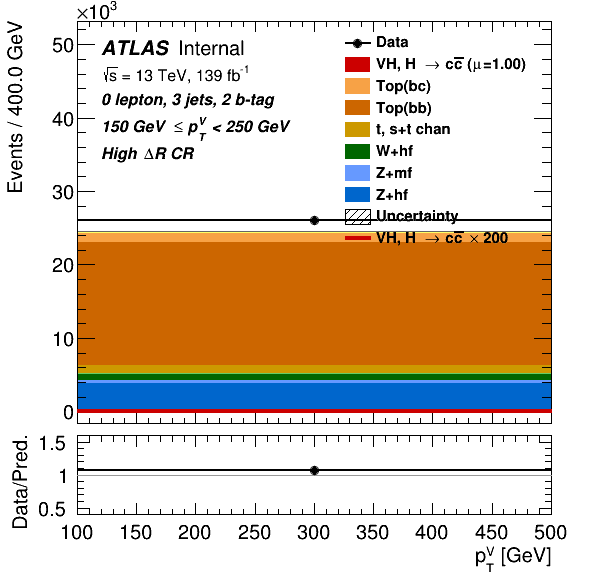
\includegraphics[width=0.48\textwidth25]{Images/VH/SRsandTopCRs/Region_distpTV_DCRHigh_BMax250_L0_Y6051_TTypebb_T2_J3_BMin150_Prefit.png}
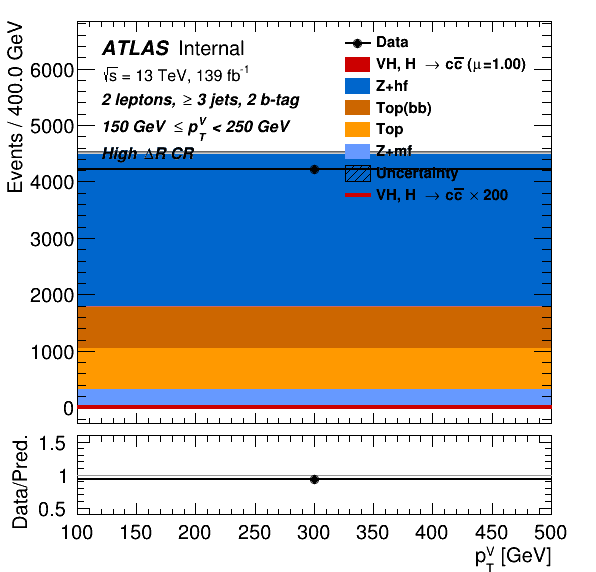
\includegraphics[width=0.48\textwidth25]{Images/VH/SRsandTopCRs/Region_distpTV_DCRHigh_BMax250_BMin150_Y6051_TTypebb_T2_J3_L2_incJet1_Prefit.png}
\caption{The $VH(H\rightarrow b\bar{b})$ High $\Delta R$ CR in the [150, 250] GeV $p_T^V$ range region with 3 jets, for 0L on the left, and 2L on the right.} 
\label{fig:vhbbDRCR02L}
\end{figure}

For $VH(H\rightarrow c\bar{c})$, the $bc$ and $bl$ components are the most important to constrain. In $VH(H\rightarrow b\bar{b})$, while the $bc$ component is also significant and can benefit from the topCRs, the most important contribution comes from the $bb$ one and is well constrained by the High $\Delta R$ CR, since in a $t\bar{t}$ decay the two produced $b$-jets tend to be separated by a large $\Delta R$ due to the event topology. For the Combined Analysis, the SRs and CRs of both analyses will be considered simultaneously. To show the impact on the $VH(H\rightarrow c\bar{c})$ standalone analysis, the High $\Delta R$ CR from  $VH(H\rightarrow b\bar{b})$ is included to study the effect on the $bc$ and $bl$ components. The aim is to demonstrate these and the $bb$ component can be well constrained with these regions alone, and in particular without the SRs of $VH(H\rightarrow b\bar{b})$. The $VH(H\rightarrow b\bar{b})$ High $\Delta R$ control regions are taken as a single bin of $p_T^V$, because the interest is solely to constrain the top($bb$) normalisation. Figure~\ref{fig:vhbbDRCR} displays the 1L $VH(H\rightarrow b\bar{b})$ High $\Delta R$ CR, which is visibly dominated by the top($bb$). Figure~\ref{fig:vhbbDRCR02L} shows the same region for the [150, 250] GeV $p_T^V$ range with 3 jets in 0L and 2L, showing a significant proportion of $Z$+jets is also included in these regions.  \\
